\documentclass[a4paper]{report}
\renewcommand{\baselinestretch}{1.5} 

%% Language and font encodings
\usepackage[utf8]{inputenc}
\usepackage[T1]{fontenc}
\usepackage[square,sort&compress]{natbib}    
\usepackage{booktabs}
\usepackage[french,english]{babel}
%% Sets page size and margins
\usepackage[top=1in,left=1.5in,bottom=1in,right=1in]{geometry}

\usepackage{relsize}
%% Useful packages
\usepackage{amsmath, amssymb}
\usepackage{graphicx}
\usepackage{subfig}

\usepackage[
	bookmarks       = true,             % Show the bookmarks
	unicode         = true,             % Use Unicode                 
	pdftoolbar      = true,             % Show Acrobat’s toolbar
	pdfmenubar      = true,             % Show Acrobat’s menu
	pdffitwindow    = false,            % Window fit to page when opened
	pdfstartview    = {FitH},           % Fit the page width to the window
	pdfnewwindow    = true,             % Open the links in a new PDF window 
	colorlinks      = true,             % Use colored links
	linkcolor       = blue,             % Internal links color
	citecolor       = blue,            % Bibliographic links color
	filecolor       = cyan,             % File links color
	urlcolor        = magenta            % External links color
]{hyperref}
\usepackage{algorithm}
% \usepackage{algorithmic}
\usepackage{algorithmicx}
\usepackage{listings}
\usepackage{algcompatible}
\usepackage{algpseudocode}
\usepackage{tikz}
\usepackage{calc}

\usepackage{pgfplots}
\usepackage{pdfpages}
\pgfplotsset{compat=1.14}
\usepackage{tikzducks}
\usetikzlibrary{snakes}
\usetikzlibrary{positioning}
\usetikzlibrary{shapes,arrows,arrows.meta}
\usetikzlibrary{automata,arrows,positioning,calc}

\usetikzlibrary{matrix}
% \usepackage{cmbright}

\makeatletter
\newcounter{algorithmicH}% New algorithmic-like hyperref counter
\let\oldalgorithmic\algorithmic
\renewcommand{\algorithmic}{%
  \stepcounter{algorithmicH}% Step counter
  \oldalgorithmic}% Do what was always done with algorithmic environment
\renewcommand{\theHALG@line}{ALG@line.\thealgorithmicH.\arabic{ALG@line}}
\makeatother

% \geometry{inner=1cm, outer=1cm, top=1cm, bottom=0cm}
\newcommand\fillin[1]{\makebox[#1]{\dotfill}}
% Use a modern font (that is not pixelated)
\usepackage{kpfonts}
% Use microtype to improve readability
\usepackage[protrusion = true, expansion = true]{microtype} 
% Use multiple columns
\usepackage{multicol}
% \usepackage{subfigure}
% \usepackage[subfigure]{tocloft}
% Display list of Equations
% \usepackage{tocloft}
% Insert empty pages
% \usepackage{afterpage}
% Configure style aspects of the document
\usepackage{caption}            % To configure the captions
\usepackage{siunitx}            % For SI units
\usepackage{graphicx}           % To include graphics
% \usepackage[dvipsnames]{xcolor} % To configure colors
\usepackage{fancyhdr}           % To configure the header and footer
% \pagestyle{fancy}               % Use a fancy header style
% \fancyhf{}                      % Set the header format
% \fancyheadoffset{0.0 cm}        % Set the header offset
\lhead{\tfm}                    % Set the header right-side contents
\rhead{\name}                   % Set the header left-side contents
% \cfoot{\thepage}                % Set the footer page number
\usepackage{amsthm}
\usepackage[capitalise,nameinlink,noabbrev]{cleveref}
\crefname{equation}{}{}
\crefname{enumi}{}{}


\newtheorem{lemma}{Lemma}
\newtheorem{theo}{Theorem}
\newtheorem{coro}{Corollary}
\newtheorem{prop}{Proposition}
\newtheorem{property}{Property}
\newtheorem{remark}{Remark}
\newtheorem{ex}{Example}
\newtheorem{exercise}{Exercise}
\newtheorem{definition}{Definition}
\newtheorem{hp}{Assumption}

% Distributions.
\newcommand*{\UnifDist}{\mathsf{Unif}}
\newcommand*{\ExpDist}{\mathsf{Exp}}
\newcommand*{\DepExpDist}{\mathsf{DepExp}}
\newcommand*{\GammaDist}{\mathsf{Gamma}}
\newcommand*{\LognormalDist}{\mathsf{LogNorm}}
\newcommand*{\WeibullDist}{\mathsf{Weib}}
\newcommand*{\ParetoDist}{\mathsf{Par}}
\newcommand*{\NormalDist}{\mathsf{Normal}}

\newcommand*{\GeometricDist}{\mathsf{Geom}}
\newcommand*{\NegBinomialDist}{\mathsf{NegBin}}
\newcommand*{\BinomialDist}{\mathsf{Bin}}
\newcommand*{\PoissonDist}{\mathsf{Poisson}}

% Sets of numbers.
\newcommand*{\RL}{\mathbb{R}}
\newcommand*{\N}{\mathbb{N}}
\newcommand*{\NZ}{\mathbb{N}_0}
% \newcommand*{\NL}{\mathbb{N}_+}

\newcommand*{\cond}{\mid}
\newcommand*{\given}{\,;\,}

%Probability symbols
\newcommand*{\Prob}{\mathbb{P}}
\newcommand*{\Q}{\mathbb{Q}}
\newcommand*{\E}{\mathbb{E}}
\newcommand*{\V}{\mathbb{V}}
\newcommand*{\F}{\mathcal{F}}
\newcommand*{\Data}{\mathcal{D}}

% Regarding spacing and abbreviations.
\usepackage{xspace}

% Acronyms
% \@\xspace doesn't add space if next char is punctuation
% However, these will give 2 .'s if used at end of sentence.
\newcommand*{\eg}{e.g.\@\xspace}
\newcommand*{\ps}{p.s.\@\xspace}
\newcommand*{\ie}{i.e.\@\xspace}
\newcommand*{\va}{v.a.\@\xspace}
\newcommand*{\iid}{i.i.d.\@\xspace}
\newcommand*{\ssi}{s.s.i.\@\xspace}
\newcommand*{\cf}{c.f.\@\xspace}
\newcommand*{\pdf}{p.d.f.\@\xspace}
\newcommand*{\pmf}{p.m.f.\@\xspace}
\newcommand*{\cdf}{c.d.f.\@\xspace}
\newcommand*{\SMC}{\textbf{SMC}\@\xspace}
\newcommand*{\MCMC}{\textbf{MCMC}\@\xspace}
\newcommand*{\VF}{\textbf{VF}\@\xspace}


\newcommand*{\iidSim}{\overset{\mathrm{i.i.d.}}{\sim}}
\newcommand*{\bt}{\bm{\theta}}
\newcommand*{\bTheta}{\bm{\Theta}}
\newcommand*{\bbeta}{\bm{\beta}}
\newcommand*{\bx}{\mathbf{x}}
\newcommand*{\bs}{\bm{s}}
\newcommand*{\bu}{\bm{u}}
\newcommand*{\bn}{\bm{n}}

% Roman versions of things.
\newcommand*{\dd}{\mathop{}\!\mathrm{d}}
\newcommand*{\e}{\mathrm{e}}
\DeclareMathOperator*{\argmax}{arg\,max}
\DeclareMathOperator*{\argmin}{arg\,min}

\newcommand*{\norm}[1]{\lVert{} #1\rVert}

% \DeclarePairedDelimiterXPP{\ind}[1]{\ind_}{\{}{\}}{}{#1}
\newcommand*{\ind}{\mathbb{I}}
\newcommand{\ra}[1]{\renewcommand{\arraystretch}{#1}}
% \addto\captionsfrench{\def\tablename{{Tableau}}}
\makeatletter

\makeatother
\begin{document}
% \frontmatter
\title{Modèles de durée\\
[0.2em]\smaller{}M1 DUAS - Université de Strasbourg}
\author{Pierre-O Goffard}

\date{updated on \today} 
\maketitle
\tableofcontents
% !TEX root = ../main_lecture_notes.tex
\chapter{Introduction}\label{sec:introduction}
Les modèles de durée permettent l'étude statistique du temps avant qu'un évènement ne se produise, par exemple la mort d'un organisme en biologie ou la défaillance d'un composant dans un système mécanique. La modélisation de la durée est un problème récurrent en assurance, branche au sein de laquelle on s'intéresse par exemple à la
\begin{itemize}
    \item Durée de vie humaine
    \item Durée d'un arrêt de travail
    \item Durée entre deux sinistres
    \item Durée dans un état incapacité ou d'invalidité 
    \item Temps avant le défaut d'un emprunteur
\end{itemize}
% L'analyse de survie vise à répondre à des questions du type
% \begin{itemize}
%     \item Quel proportion de la population sera toujours en vie après une certaine date?
%     \item Parmi ceux qui ont survécu, à quel taux vont-ils nous quitter?
%     \item Plusieurs causes de sortie peuvent-elles être prise en compte? Par exemple dans le cadre d'un contraat d'asssurance vie de type épargne un assuré peut sortir du portefeuille pour décès ou en cas de rachat. 
%     \item Comment certaines circonstances de l'évènement ou caractéristiques indivivuelles impactent-t-elles la durée de vie?
%     \begin{itemize}
%     \item le genre
%     \item l'âge
%     \item être fumeur ou non
%   \end{itemize}
% \end{itemize}
Les tables de mortalité, de rachat ou de maintien en capacité sont issus d'analyse de survie et sont en entrée des modèles actuarielles de valorisation des portefeuilles et de gestion des risques. 
\begin{ex}
Prenons l'exemple d'un contrat d'assurance emprunteur. Ce contrat permet une indemnisation du prêteur (la banque) en cas de défaut de paiement de l'assuré. Il permet également une indemnisation de l'emprunteur en apportant un complément en cas de perte de revenu par exemple en cas d'arrêt de travail. L'assuré peut également résilier son contrat ou racheter son prêt. Ces différentes situations doivent être prise en compte par l'actuaire et font intervenir plusieurs modèles de durée. Le parcours de l'assuré et les hypothèse sont résumées sur la \cref{fig:schema_emprunteur}.
 \begin{figure}[h!]
 \begin{center}
\begin{tikzpicture}[->, >=stealth', auto, semithick, node distance=4cm]
% \tikzstyle{every state}=[fill=white,draw=black,thick,text=black,scale=0.8]
\tikzstyle{every state}=[rectangle,draw,rounded corners=4pt,fill=white]
\tikzstyle{test}=[diamond, aspect=2.5,thick, draw=blue,fill=yellow!50,text=blue] 

\node[test]    (1)               {$\text{Valide}$};
\node[state]    (2)[right of=1]   {$\text{Incapacité}$};
\node[state]    (3)[right of=2]   {$\text{Invalidité}$};
\node[state]    (4)[left of=1]   {$\text{Perte d'emploi}$};
\node[state]    (5)[above of=1]   {$\text{Résiliation}$};
\node[state]    (6)[left of=5]   {$\text{Rachat}$};
\node[test]    (7)[below of=2]   {$\text{Terme du prêt}$};
\node[state]    (8)[below of=1]   {$\text{Décès}$};
\path
(1) edge[bend left] node[above]{$\text{loi d'entrée en incapacité}$} (2)
(1) edge[bend left] node[below left]{$\text{loi d'entrée en chômage}$} (4)
(1) edge[left]  node{$\text{loi de mortalité}$} (8)
(1) edge[left]  node{$\text{loi de rachat}$} (6)
(1) edge[bend left]  node[right]{$\text{loi de résiliation}$} (5)
(1) edge[left]  node{} (7)
(2) edge[bend right] node{$$}  (1)
(2) edge[bend left]  node{$\text{loi d'entrée en invalidité}$}  (3)
(4) edge[bend right] node{}  (1)
(2) edge[loop below] node{$\text{loi de maintien}$} (2);
\end{tikzpicture}
\end{center}
\caption{Parcours assuré dans le cadre d'un contrat d'assurance emprunteur}
\label{fig:schema_emprunteur}
\end{figure}
\end{ex}
\section{Distribution d'une durée}
\subsection{Formulation continue}
 Une durée $T$ est une \va sur $\RL_+$ caractérisée part sa densité de probabilité $f$. On s'intéresse en particulier à la fonction de répartition 
$$
F(t)=\Prob(T\leq t) = \int_0^t f(s)\text{d}s,
$$ 
et à sa fonction de survie $S(t) = \Prob(T>t)$. La moyenne de $T$ est donnée par 
$$
\E(T) = \int_0^\infty t f(t)\text{d}t = \int_0^\infty S(t)\text{d}t.
$$
La fonction de survie conditionnellement à la survie jusqu'a l'instant $u$ est donnée par 
$$
S_u(t) = \Prob(T> t+u|T>u) = \frac{\Prob(T> t+u)}{\Prob(T>u)} = \frac{S(u+t)}{S(u)}.
$$
La fonction de hasard $h$\footnote{aussi appelé taux de panne, taux de décès, taux de défaillance suivant le contexte} est donnée par 
$$
h(t) =\frac{\Prob[T\in(t,t+\text{d}t)|T>t]}{\text{d}t}= \frac{f(t)}{S(t)}= -\frac{S'(t)}{S(t)} = -\frac{\text{d}}{\text{d}t}\ln S(t).
$$
Il s'agit de la probabilité que l'évènement se produise à $t$ sachant qu'il ne s'est pas produit avant. On définit également la fonction de hasard cumulé par 
$$
H(t) = \int_0^th(s)\text{d}s.
$$
On note que 
$$
S(t) = \exp[-H(t)].
$$
% Dans certains tests d'adéquation statistique on utilise le fait que la \va $H(T)$ suive une loi exponetielle. En effet, 
% $$
% \Prob[H(T)>t)] = \Prob[T>H^{-1}(t)]=S(H^{-1}(t)) = \exp[-H(H^{-1}(t))] = e^{-t}
% $$
La fonction de survie conditionelle est donnée en terme de la fonction de hasard cumulée par 
$$
S_u(t) = \exp\left[-\int_u^{t+u}h(s)\text{d}s\right] = \exp\left[-(H(u+t)-H(u))\right].
$$
\subsection{Formulation discrète}
Il arrive que $T$ est exprimé en nombre d'heure, nombre de jour, ou nombre d'année. Cela rend possible la modèlisation par une \va à valeur dans $\N$, caractérisée par sa loi de probabilité 
$$
p(k) = \Prob(T=k),\text{ }k\in\N.
$$
La fonction de survie est donnée par 
$$
S(k) = \sum_{l\geq k+1}^\infty p(l).
$$
On définit, de manière équivalente au cas continu, la fonction de hasard avec 
$$
h(k) = \Prob(T = k|T>k-1) = \frac{p(k)}{S(k-1)},\text{ }k\geq 1.
$$
On note que 
\begin{eqnarray*}
S(k) &=& \Prob(T>k)\\
&=& \Prob(T>k|T>k-1)S(k-1)\\
&=& [1-\Prob(T\leq k|T>k-1)]S(k-1)\\
&=& [1-\Prob(T= k|T>k-1)]S(k-1)\\
&=& [1-h(k)]S(k-1)\\
&\vdots&\\
&=&\prod_{l=0}^k[1-h(l)].
\end{eqnarray*}
\begin{remark}
Dans l'étude de la mortalité, la variable $T$ correspond à l'âge de décès et on note 
$$
q_x = h(x) = \Prob(T=x|T> x-1) = \frac{\Prob(T=x)}{S(x-1)},
$$
la probabilité de décès à l'âge $x$.
\end{remark}

\subsection{Le passage du continu au discret et inversement}
Pour une variable $T$ continue, on peut discrétiser en considérant que $T=k\epsilon$ lorsque $k\epsilon\leq T <(k+1)\epsilon$, ce qui revient à remplacer $T$ par $\epsilon\lfloor T/\epsilon\rfloor$. $\epsilon$ est le pas de discrétisation. Le passage du discret au continu se fait par interpolation des fonctions de survie ou de hasard.

% \section{Un premier exemple: Durée d'un arrêt de travail}

% On étudie l'entrée et le maintien en incapacité au sein d'une population d'assuré sont étudié sur la période allant du $01/01/203$ au $31/12/2008$. Le tableau \cref{tab:incap_data} montre les $5$ premières observations  du jeu de données
% % latex table generated in R 4.2.1 by xtable 1.8-4 package
% % Sun Dec  4 15:33:26 2022
% \begin{table}[ht]
% \centering
% \scriptsize
% \begin{tabular}{lllllllll}
%   \hline
%   Sexe & CSP & ModeSouscription & TypeArret & DateNaissance & DateSurvenance & DateEntree & DateSortie & MotifReprise \\ 
%   \hline
%  H & NCA & NONCSPEC & Accident du travail & 1962-12-06 & 2006-10-07 & 2006-11-04 & 2006-11-13 & 3 - Termine \\ 
%   F & ENP & NONCSTAN & Maladie & 1969-01-01 & 2006-08-05 & 2006-08-05 & 2006-09-10 & 3 - Termine \\ 
%   F & ENP & NONCSTAN & Maladie & 1969-01-01 & 2005-01-14 & 2005-01-14 & 2005-01-30 & 3 - Termine \\ 
%   F & ENP & NONCSTAN & Maladie & 1969-01-01 & 2005-11-18 & 2006-01-01 & 2006-01-01 & 3 - Termine \\ 
%   F & CAD & NONCSTAN & Maladie & 1958-01-02 & 2004-06-01 & 2005-10-26 & 2005-11-30 & 2 - Invalide \\ 
%    \hline
% \end{tabular}
% \caption{Extrait du jeu de incapacité}
% \label{tab:incap_data}
% \end{table}
% Ce jeu de données comprends $560,725$ lignes, chaque observations correspond à une entrée en incapacité avec potentiellement plusieurs évènements par individus. Le jeu de données contient $9$ variables 
% \begin{itemize}
%  \item Sexe
%  \item CSP
%  \item ModeSouscription
%  \item TypeArret =  S'agit-t-il d'un acident du travail ou d'un arrêt maladie
%  \item dateNaissance
%  \item DateSurvenance = date de déclenchement de l'entrée en incapacité
%  \item DateEntree =  date de début d'indemnisation
%  \item DateSortie = date de fin d'indemnisation
%  \item MotifReprise = raison de fin d'incapacité
% \end{itemize}
% On peut représenter les données comme sur la \cref{fig:INC_visu}. 
% \begin{figure}[h!]
% \centering
% 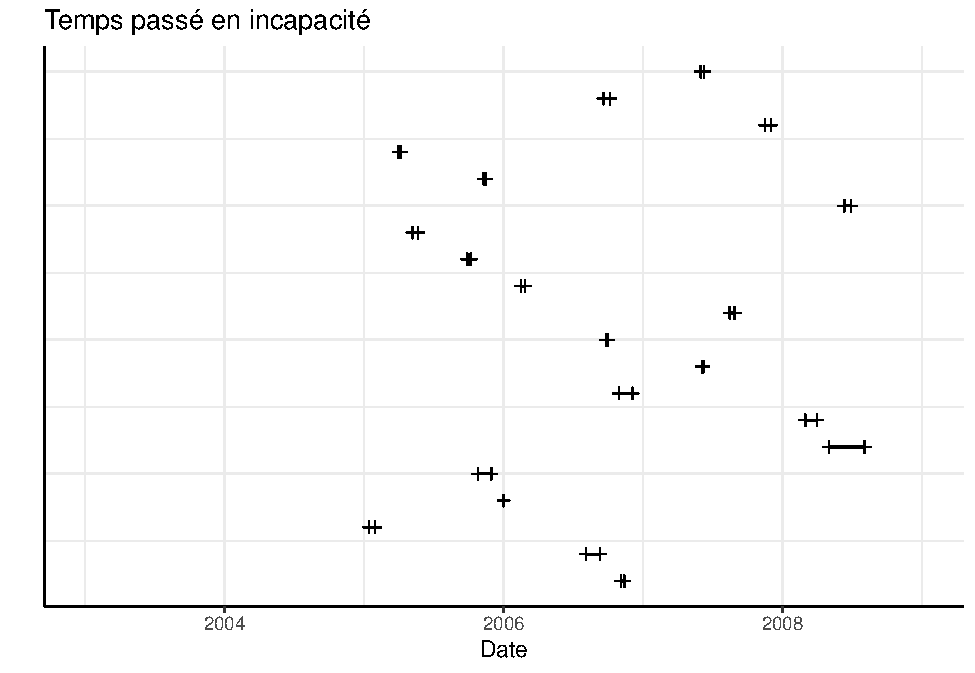
\includegraphics[width = 0.7\textwidth]{../figures/INC_visu}
% \caption{Occurence et longueur des arrêts de travail par individu}
% \label{fig:INC_visu}
% \end{figure}
% Chaque ligne de la \cref{fig:INC_visu} correspond à une entrée en incapacité et nous observons l'occurence et la temps passé en incapacité. Nous avons
% \begin{itemize}
% \item des données répétées, c'est à dire potentiellement plusieurs enrée en incapacité pour un même individu
% \item des données censurées droite, c'est à dire des arrêts de travail qui se sont poursuivis après la date de fin d'observation (ici au $31/12/2008$)
% \item des données censurées à gauche, des arrêts de travail qui ont débuté avant la date de début d'observations (ici au $04/01/2003$)
% \item des données tronqués, si par exemple les arrêts de travail inférieur à 3 jours sont exclus ou non observable. Cela arrive en pratique si un délai de carence est appliqué. On peut aussi considérer qu'au delà de trois mois l'arrêt de travail est requalifié en "arrêt de travail longue durée" entrainant une mise en réduction des garanties. Dans ce cas on exclus les arrêts de travails supréieurs à trois mois de l'étude.
% \item des covariables, qui peuvent influencer le temps passé en incapacité par exemple est ce que l'entrée en incapacité est du à un accident du travail ou une maladie.
% \end{itemize}




\section{Modélisation statistique}
Soient $t_1,\ldots, t_n$ des réalisations \iid de la variable $T$. Les données disponibles pour l'analyse de survie sont souvent incomplètes, on est ainsi confronter au problème de censure et de troncature comme illustré sur la \cref{fig:censored_truncated_data}. 

\begin{figure}
\begin{center}
\begin{tikzpicture}[scale=1, every node/.style={scale=1}]
    % Draw axes
    \draw [<->,thick] (0,11) node (yaxis) [above] {}
        |- (10,0) node (xaxis) [right] {Duration};

    % Draw vertical lines for observed durations
    \foreach \y/\xstart/\xend/\type in {
        1/1/4/observed,
        1/5/6/truncated,
        2/2/7/l_censored,
        3/1/2/truncated,
        4/0.5/4/observed,
        5/3/6/r_censored,
        6/2/3/truncated,
        7/1/3/observed,
        7/5/7/r_censored,
        8/1.5/7/r_censored,
        9/2.5/3/truncated,
        10/0.3/3.5/observed}{
        % Dotted line for truncated data
        \ifthenelse{\equal{\type}{truncated}}{
            \draw [thick, densely dotted] (\xstart,\y) -- (\xend,\y);
        }{}
        % Solid line with bullet points for observed data
        \ifthenelse{\equal{\type}{observed}}{
            \filldraw (\xstart,\y) circle (2pt);
            \draw [thick] (\xstart,\y) -- (\xend,\y);
            \filldraw (\xend,\y) circle (2pt);
        }{}
        % Solid line with bullet point at the start and parenthesis at the end for censored data
        \ifthenelse{\equal{\type}{r_censored}}{
            \filldraw (\xstart,\y) circle (2pt);
            \draw [thick, dashed] (\xstart,\y) -- (\xend,\y);
            % \draw (\xend,\y) +(-2pt,-2pt) rectangle +(4pt,4pt);
            \node at (\xend,\y) [star, star points=5, star point ratio=2.25, fill, inner sep=1.5pt] {};
            % \draw [thick] (\xend,\y) -- (\xend+0.5,\y) node[right] {};
            % \draw (\xend,\y)++(2pt,2pt) -- ++(0,-4pt) arc (-90:90:2pt) -- cycle;
        }{}
        \ifthenelse{\equal{\type}{l_censored}}{
            \node at (\y,\xstart) [star, star points=5, star point ratio=2.25, fill, inner sep=1.5pt] {};
            \draw [thick, dashed] (\xstart,\y) -- (\xend,\y);
            \filldraw (\xend,\y) circle (2pt);
        }{}
    }

    % Optionally, add a legend
    \filldraw (11,6) circle (2pt) -- (12,6) circle (2pt) node[right] {\,Observée};
    \filldraw (11,5) circle (2pt);
    \draw [thick, dashed] (11,5) circle (2pt) -- (12,5) node[right] {\,Censurée à droite};
    \node at (12,5) [star, star points=5, star point ratio=2.25, fill, inner sep=1.5pt] {};
    \draw [thick, densely dotted] (11,3) -- (12,3) node[right] {\,Tronquée à gauche};
    % \node at (11,4) [star, star points=5, star point ratio=2.25, fill, inner sep=1.5pt] {};
    % \filldraw (12,4) circle (2pt);
    % % \draw [thick, dashed] (11,4) -- (12,4) circle (2pt) node[right] {\,Censurée à gauche};
    

\end{tikzpicture}
\end{center}
\caption{Illustration des phénomènes de censure, de troncature et de données répétées}
\label{fig:censored_truncated_data}
\end{figure}

Chaque ligne de la \cref{fig:censored_truncated_data} correspond à un évènement et nous observons l'occurence et la durée de chaque évènement. Nous avons
\begin{itemize}
\item des données répétées, c'est à dire potentiellement plusieurs évènement pour un même individu
\item des données censurées droite, c'est à dire des évènements observé jusqu'a une certaine date 
\item des données censurées à gauche, c'est à dire des évènements observé depuis une certaine date 
\item des données tronqués, ici des évènements qui n'ont pas duré assez longtemps pour être observés
\item des covariables, qui peuvent influencer la durée d'un évènement
\end{itemize}

L'objectif du cours est de proposer des méthodes d'estimation pour la fonction de survie $S$. Le \cref{chap:parametric} détaille l'aproche paramétrique consiste à supposer que la distribution de $T$ appartient à une famille de distributions paramétriques, c'est à dire que $S(t) := S(t;\theta)$. L'objectif est de trouver la valeur du paramètre $\widehat{\theta}$ permettant le meilleur ajustement du modèle aux données.  N'importe quelle loi de probabilité sur $\mathbb{R}_+$ ou sur $\mathbb{N}$ peut convenir. Le \cref{chap:nonparametric} présente les approches non paramétriques dans lesquelles on ne fait pas l'hypothèse d'un modèle sous-jacent, l'estimateur $\widehat{S}(t)$ est totalement \textit{data-driven}. Le \cref{chap:Ph_models} présente des méthodes pour étudier la distribution de $T$ conditionnellement à des covariable $Z$. Les évènements étudiés sont caractérisé par un vecteur $Z$ d'information externe ayant un impact supposé sur la durée de l'évènement. Le \cref{chap:mortality_table}
introduit des modèles actuariels (aussi étudié en démographie) pour étudié la mortalité des individus au sein d'un population (ou d'un portefeuille d'assurés). 
%  En prenant l'exemple des données d'arrêt de travail ce qui correspond à ignorer le caractère répété des observations et la potentielle censure. Le tableau \cref{tab:stat_desc_T} donne quelques statistiques descriptives.
% \begin{table}[ht]
% \centering
% \begin{tabular}{rrrrrrrrr}
%   \hline
%  & n & mean & sd & q25 & q50 & q75 & min & max \\ 
%   \hline
% $T$ & $560,725$ & $25$ & $62 $& $4$ & $10$ & $23$ & $0$ & $1440$ \\ 
%    \hline
% \end{tabular}
% \caption{Statistiques descriptives des temps passé en incapacité}
% \label{tab:stat_desc_T}
% \end{table}
% \subsection{Approche non paramétrique}
% La distribution empirique d'une \va est souvent visualiser graphiquement au travers d'un histogramme et d'une boîte à moustache comme sur la \cref{fig:INC_hist_boxplot}.
% \begin{figure}[h!]
% \centering
% 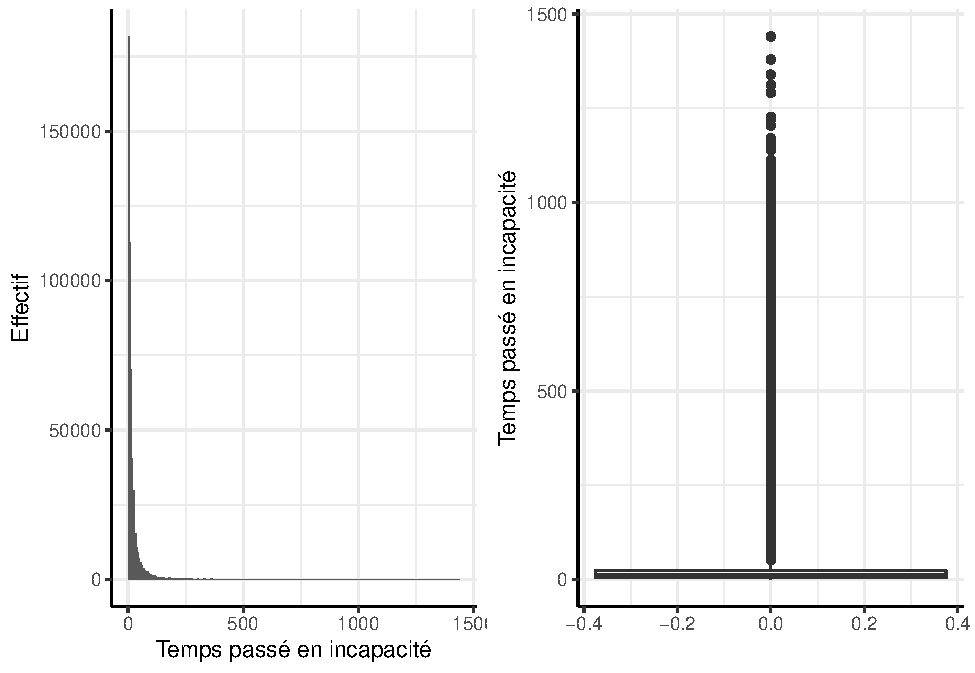
\includegraphics[width = 0.8\textwidth]{../figures/INC_hist_boxplot}
% \caption{Histogramme et boîte à moustache des $t_{i,j}$}
% \label{fig:INC_hist_boxplot}
% \end{figure}
% La hauteur des barres de l'histogramme sont données par $\sum_i \sum_j \mathbb{I}_{[kh,(k+1)h)}(t_{i,j})$, en divisant par $n$, par $h$ et en prenant $h$ petit, on retrouve une estimation de la densité de probabilité. La fonction de survie peut être estimée par sa contre partie empirique avec 
% \begin{equation}\label{eq:fonction_survie_estim_nonp}
% \widehat{S}(t) = \frac{1}{n}\sum_{i=1}^n\mathbb{I}_{t_{i} > t}.
% \end{equation}
% De même pour la fonction de hasard cumulé avec
% $$
% \widehat{H}(t) = -\ln \widehat{S}(t).
% $$
% Les estimations obtenues sont reportées sur la \cref{fig:INC_S_H_nonp}.
% \begin{figure}[h!]
% \centering
% 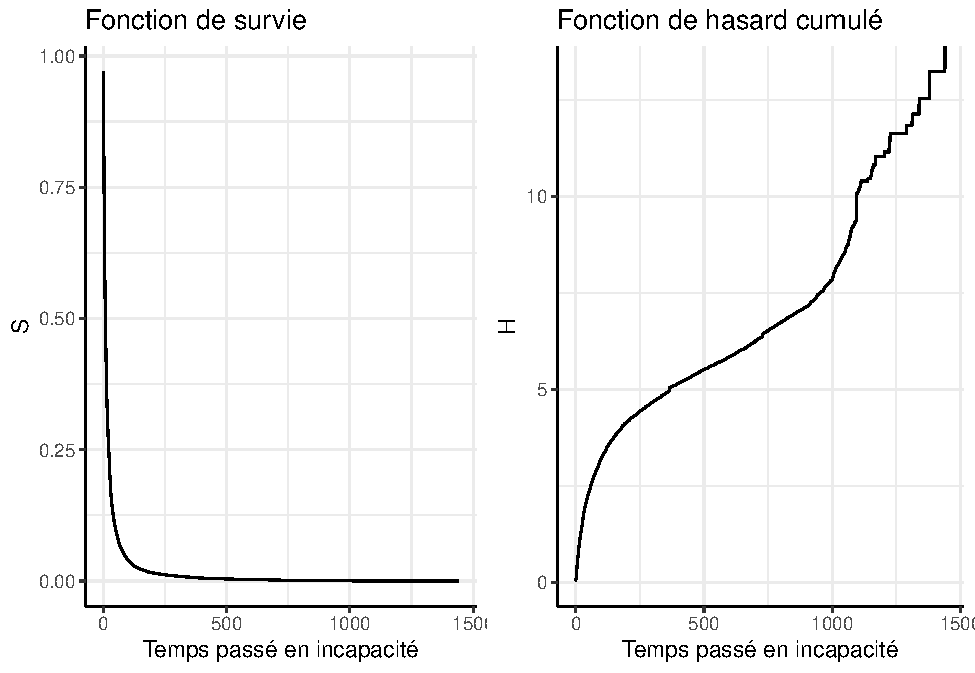
\includegraphics[width = 0.8\textwidth]{../figures/INC_S_H_nonp}
% \caption{Fonction de survie et de hasard cumulée estimées non paramétriquement.}
% \label{fig:INC_S_H_nonp}
% \end{figure}
% Nous verrons plus tard comment prendre en compte l'occurence de valeur censurée / tronquée dans l'écriture des estimateurs. L'utilisation de l'estimateur \eqref{eq:fonction_survie_estim_nonp} nécessiterait de retirer les valeurs censurées de l'étude. Si la variable aléatoire $T$ est considérée comme discrètes, on peut estimer les taux de sortie de l'état d'incapacité par 
% $$
% \widehat{h}(t) = \frac{\sum_{i=1}^n\mathbb{I}_{t_{i} = t}}{\sum_{i=1}^n\mathbb{I}_{t_{i} \geq t}}.
% $$
% La série des taux de sortie est donnée sur la \cref{fig:INC_h_nonp}.
% \begin{figure}[h!]
% \centering
% 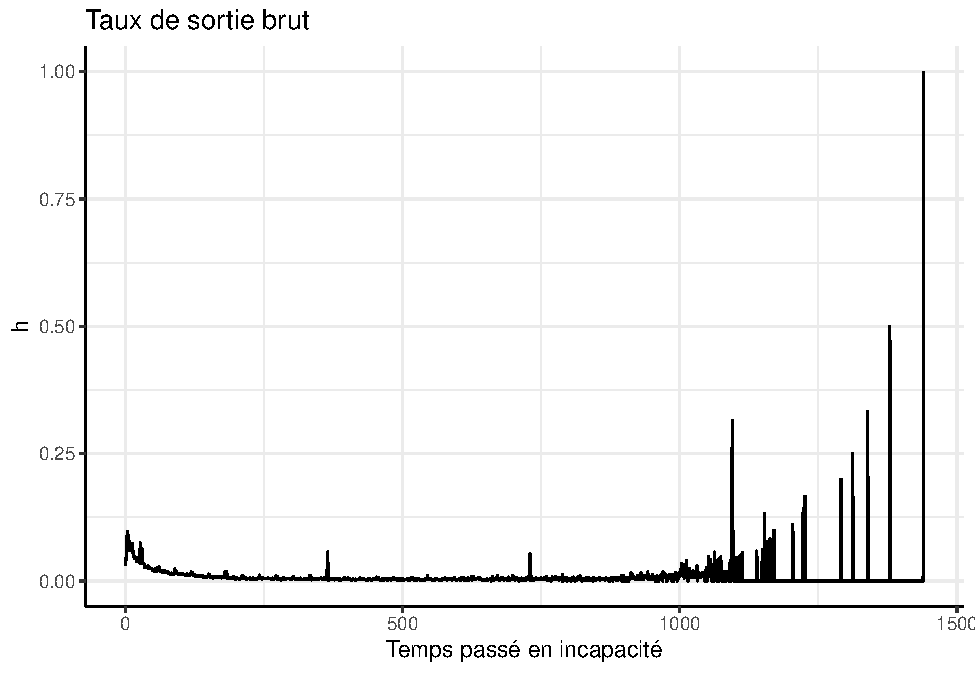
\includegraphics[width = 0.8\textwidth]{../figures/INC_h_nonp}
% \caption{Fonction de hasard estimée non paramétriquement via l'estimateur empirique.}
% \label{fig:INC_h_nonp}
% \end{figure}
% L'aspect un peu erratique de ces taux de sortie "brut" est souvent corrigé par l'application d'une méthode de lissage.
% \subsection{L'approche paramétrique}
% L'aproche paramétrique consiste à supposer que la distribution de $T$ appartient à une famille de distributions paramétriques, c'est à dire que $S(t) := S(t;\theta)$. L'objectif est de trouver la valeur du paramètre $\widehat{\theta}$ permettant le meilleur ajustement du modèle aux données.  N'importe quellle loi de probabilité sur $\mathbb{R}_+$ ou sur $\mathbb{N}$ peut convenir. Pour l'exemple, prenons la loi exponentielle $\text{Exp}(1/\mu)$ (telle que $\mathbb{E}[\text{Exp}(\mu)] = \mu$) et la loi de poisson $\text{Pois}(\lambda)$. L'estimation est très facile pour ces lois comme 
% $$
% \widehat{\mu} = \widehat{\lambda} = \frac{1}{n}\sum_{i=1}^nt_i.
% $$
% Nous pouvons vérifier l'adéquation en superposant les graphiques des fonctions théoriques et empiriques comme sur la \cref{fig:INC_S_H_p}.
% \begin{figure}[h!]
% \centering
% 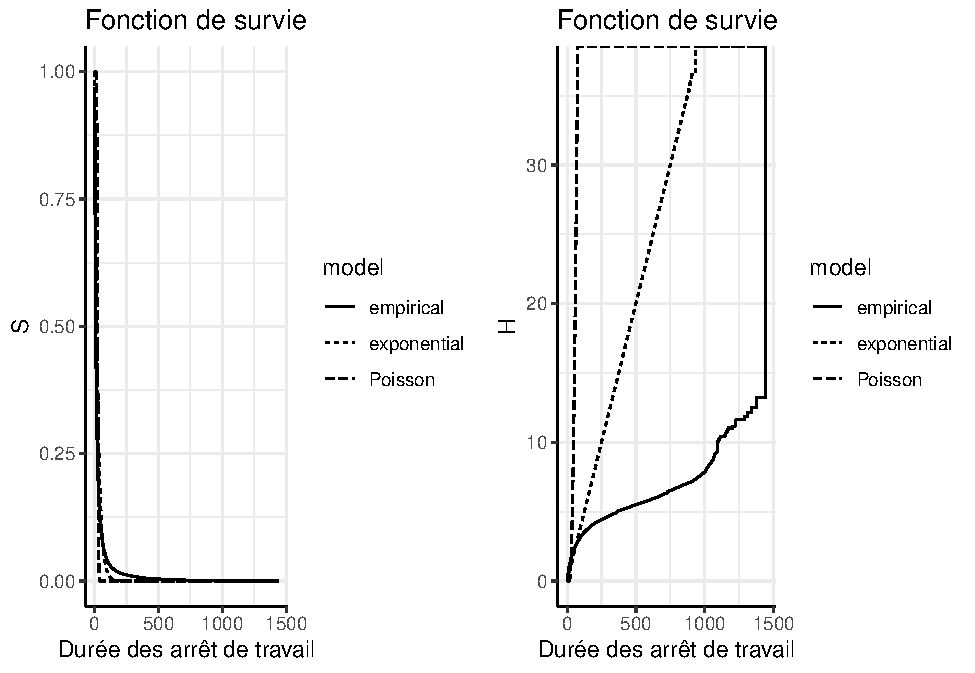
\includegraphics[width = 0.8\textwidth]{../figures/INC_S_H_p}
% \caption{Fonction de survie et de hasard cumulée estimées non paramétriquement.}
% \label{fig:INC_S_H_p}
% \end{figure}
% L'adéquation n'est pas optimale, nous étudierons des modèles paramétrique plus adaptés et nous verrons également des modèles dit semi-paramétriques permetttant un arbitrage entre des hypothèses fortes (paramétrique) et une grande fléxibilité (modèle non paramétrique). L'intérêt de ces modèles réside aussi dans l'ajout de covariables qui est discuté ci-après.
% \section{Ajout de facteurs explicatifs}
% La survie des individus ou des composants peut s'expliquer par les caractéristiques des individus ou des circonstances exogènes qui peuvent être connu grâce à des covariables ou variables explicatives, notées $X$. La variable $T$ est la variable à expliquer et on s'interesse à la loi conditionnelle de $T$ sachant $X$. Dans notre exemple, nous nous servirons de la variable \texttt{TypeArret} qui indique le motif de l'enrée en incapacité. Le tableau \cref{tab:stat_desc_by_TypeArret} reporte les statistiques descriptives de la durée des arrêts de travail en fonction du traitement reçu.  
%  \begin{table}[ht]
% \centering
% \begin{tabular}{l|rrrrrrrr}
%   \hline
%   TypeArret & n & mean & sd & q25 & q50 & q75 & min & max \\ 
%   \hline
% Accident du travail & 64295 & 26 & 60 & 5 & 12 & 25 & 0 & 1379 \\ 
%  Maladie & 496107 & 25 & 62 & 4 & 9 & 23 & 0 & 1440 \\ 
%  Maternite & 323 & 52 & 52 & 10 & 29 & 98 & 0 & 237 \\ 
%    \hline
% \end{tabular}
% \caption{Statistques descriptives de la durée de l'incapacité en fonction du motif d'entrée en incapacité}
% \label{tab:stat_desc_by_TypeArret}
% \end{table}
% Les distributions semblent similaires pour les incapacités liées à une maladie ou un accident du travail, nous laissrons de ôté les entrées en incapacité pour congé de maternité. La \cref{fig:INC_S_H_cohorte} permet de comparer les estimations de la fonction de survie et de hasard cumulés.
% \begin{figure}[h!]
% \centering
% 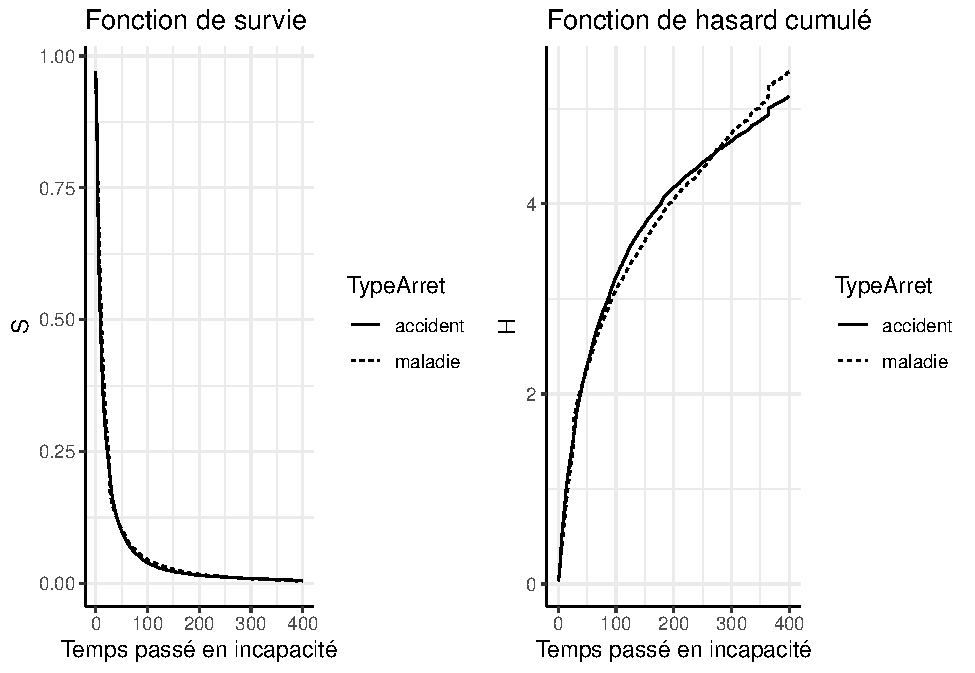
\includegraphics[width = 0.8\textwidth]{../figures/INC_S_H_cohorte}
% \caption{Fonction de survie et de hasard cumulée pour chacune des cohortes.}
% \label{fig:INC_S_H_cohorte}
% \end{figure}
% Nous verrons dans ce cours comment prendre en compte de manière approprièes (ou de manière plus sophistiquée) les covariables.



% !TEX root = ../main_lecture_notes.tex
\chapter{Approche paramétrique}\label{chap:parametric}
Soit $t_1,\ldots, t_n$ un échantillon de réalisation \iid de $T$. L'estimation paramétrique suppose que la loi de $T$ appartient à une famille de distribution caractérisée par un paramètre (vecteur de paramètres) $\theta$. la loi de $T$ est caractérisé par sa densité $f(t;\theta)$ si $T$ est continue ou sa loi $p(t;\theta)$ si $T$ est discrète. l'inférence s'effectue usuellement en maximisant la fonction de vraisemblance definie par 
$$
L(\Data;\theta) = L(t_1,\ldots, t_n;\theta) = \begin{cases}
\prod_{i}^nf(t_i;\theta),&\text{ dans le cas continu},\\
\prod_{i}^np(t_i;\theta),&\text{ dans le cas discret}.
\end{cases}
$$
Cette écriture correspond au cas où les données sont complètes. comme vu dans le chapitre précédent, ce n'est pas toujour le cas dans les analyses de survie. Nous devons distinguer plusieurs cas de données incomplètes et modifier en conséquence l' écriture de la vraisemblance. Dans la pratique, on chercher à maximiser la log-vraisemblance 
$$
l(\Data;\theta)=\log L(\Data;\theta)
$$
via des algorithmes d'optimisation numérique\footnote{Les fonctions \texttt{nlm} et \texttt{optim} en R}.

\section{Fonction de vraisemblance en présence de censure et de troncature}\label{sec:like}

\begin{definition}\label{def:censure_tronquature}
La \va $T$ est censuré à droite (resp. à gauche) si 
$$
T = C \text{ si }T\geq C (\text{resp. } T\leq C).
$$
La \va $T$ est tronquée à droite (resp. à gauche) si $T$ n'est pas observée si
$T\leq C$ (\text{resp. } $T>C$).
\end{definition}
\begin{ex}
\begin{enumerate}
\item L'étude porte sur l'âge au quel les enfant apprenne une compétence. Lorsque l'étude débute, certains enfant d'âge $C$ maitrise déjà la compétence, pour eux $T\leq C$ (censure à gauche). A la fin de l'étude d'autre enfant d'âge $C$ ne maitrise pas encore la compétence alors $T\geq C$ (censure à gauche)

\item L'étude porte sur la durée de survie $T$ de patients atteints d'une certaine maladie. Pour les patients perdus de vue
au bout du temps $C$ alors qu'ils étaient encore vivants, $C$ censure $T$ à droite puisque, pour eux, $T$ est inconnue mais supérieure à $C$.
\item L'étude porte sur la durée de vie après la retraite de sujets qui entrent dans l'enquête à la suite d'un tirage au sort dans une caisse de retraite. Un sujet n'est donc observé que si sa durée de vie après la retraite excède le délai entre sa prise de retraite et l'instant de l'enquête. La durée de vie après la retraite est donc tronquée à gauche par ce délai.
\end{enumerate}
\end{ex}
Pour plus de détails, on pourra consulter le rapport suivant \url{http://www.numdam.org/item/JSFS_1994__135_4_3_0.pdf}. Dans les applications actuarielles, on fait souvent face à des cas de censure à droite. Supposons que les niveaux de censure soient des réalisations \iid $c_1,\ldots, c_n$ d'un \va positive $C$ de densité $f_C(\cdot;\theta)$. On suppose que les \va $T$ et $C$ sont indépendantes. Les données disponibles sont
$$ 
\Data = (x_k,\delta_k)_{k=1,\ldots, n} = (t_k\land c_k,\ind_{t_k\leq c_k})_{k=1,\ldots, n}.
$$
La vraisemblance s'écrit
$$
L(\Data;\theta) = \prod_{k=1}^n[f(x_k;\theta)\cdot S_C(x_k;\theta)]^{\delta_k}[f_C(x_k;\theta)\cdot S(x_k;\theta)]^{1-\delta_k}.
$$
Il est courant que la censure n'apporte aucune information sur le paramètre du modèle $\theta$. Cela implique que $f_C(\cdot;\theta) = f_C(\cdot)$ et $S_C(\cdot;\theta) = S_C(\cdot)$. On a alors
$$
L(\Data;\theta) = \text{A}\prod_{k=1}^nf(x_k;\theta)^{\delta_k}S(x_k;\theta)^{1-\delta_k} =  A\prod_{k=1}^nh(x_k;\theta)^{\delta_k}S(x_k;\theta),
$$
où $\text{A}$ est une constante en fonction de $\theta$ qui peut être négligé dans le cadre d'une procédure d'optimisation de la vraisemblance. 
% \begin{remark}
% L'estimateur du maximum de vraisemblance obtenu dans le cadre d'une censure de type I se généralise directement à la censure de type III.
% \end{remark}
\subsection{Troncature}\label{ssec:censureIII}
Dans le cas de la troncature, une observation $t_k$ n'est disponible que si $t_k\in[c_1,c_2]$ avec $0\leq c_1< c_2\leq \infty$. La loi observé est alors la loi conditionnelle $T|T\in[c_1,c_2]$. Il faut donc remplacer $h$ et $S$ par 
$$
h_{[c_1,c_2]}(t) = \frac{S(t)h(t)}{S(t) - S(c_2)}\ind_{[c_1,c_2]}(t)
$$
et
$$
S_{[c_1,c_2]}(t) = \begin{cases}
1,&t\leq c_1\\
\frac{S(t)-S(c_2)}{S(c_1)-S(c_2)},&c_1\leq t\leq c_2,\\
0,&t> c_2.\\
\end{cases}
$$
\section{Lois paramétriques usuelles}\label{sec:common_parametric_model}
\subsection{Loi exponentielle}\label{ssec:exp}
\begin{definition}\label{def:loi_exponentielle}
Une \va $T$ de loi exponentielle $\ExpDist(\beta)$ a pour densité
$$
f(t) = \frac{\e^{- t/\beta}}{\beta}\ind_{(0,\infty)}(t),
$$ 
fonction de survie
$$
S(t) = \e^{- t/\beta},
$$
et fonction de hasard
$$
h(t) = \frac{1}{\beta}\ind_{(0,\infty)}(t).
$$
\end{definition}
\subsection{Loi Gamma}\label{ssec:gamma}
Une \va $T$ de loi gamma $\GammaDist(\alpha, \beta)$ a pour densité
$$
f(t) = \frac{t^{\alpha-1}\e^{-\beta t}}{\beta^\alpha\Gamma(\alpha)}\ind_{(0,\infty)}(t),
$$ 
où $\Gamma(\alpha) = \int_0^\infty \e^{-t}t^{\alpha-1}\text{d}t$ désigne la fonction gamma. La fonction de survie est donnée par
$$
S(t) = \frac{\Gamma_u(t/\beta, \alpha)}{\Gamma(\alpha)},
$$
où $\Gamma_u(t, \alpha) =\int_t^\infty\e^{-t}t^{\alpha-1}\text{d}t $ est la fonction gamma incomplète. La fonction de hasard est donnée par
$$
h(t) = \frac{t^{\alpha-1}\e^{-\beta t}}{\Gamma_u(t/\beta, \alpha)\beta^\alpha}\ind_{(0,\infty)}(t).
$$
\subsection{Loi de Weibull}\label{ssec:weibull}
Une \va $T$ de loi de Weibull $\WeibullDist(\alpha, \beta)$ a pour densité
$$
f(t) = \frac{\alpha}{\beta}\left(\frac{t}{\beta}\right)^{\alpha-1}\e^{-(x/\beta)^\alpha}\ind_{(0,\infty)}(t),
$$ 
fonction de survie
$$
S(t) = \e^{-(x/\beta)^\alpha},
$$
et fonction de hasard
$$
h(t) = \frac{\alpha}{\beta}\left(\frac{t}{\beta}\right)^{\alpha-1}\ind_{(0,\infty)}(t).
$$
\section{Comparaison et sélection d'un modèle}
Les trois modèles ont des caractértistiques très différentes. Les fonctions de densité, de survie, de hasard et de hasard cumulée des modèles $\ExpDist(\beta = 1)$, $\GammaDist(\alpha = 2, \beta = 1/2)$ et $\WeibullDist(\alpha = 1 / 2, \beta = 1/2)$ sont données sur la \cref{fig:d_S_h_H_parametric}.
\begin{figure}[h!]
\centering
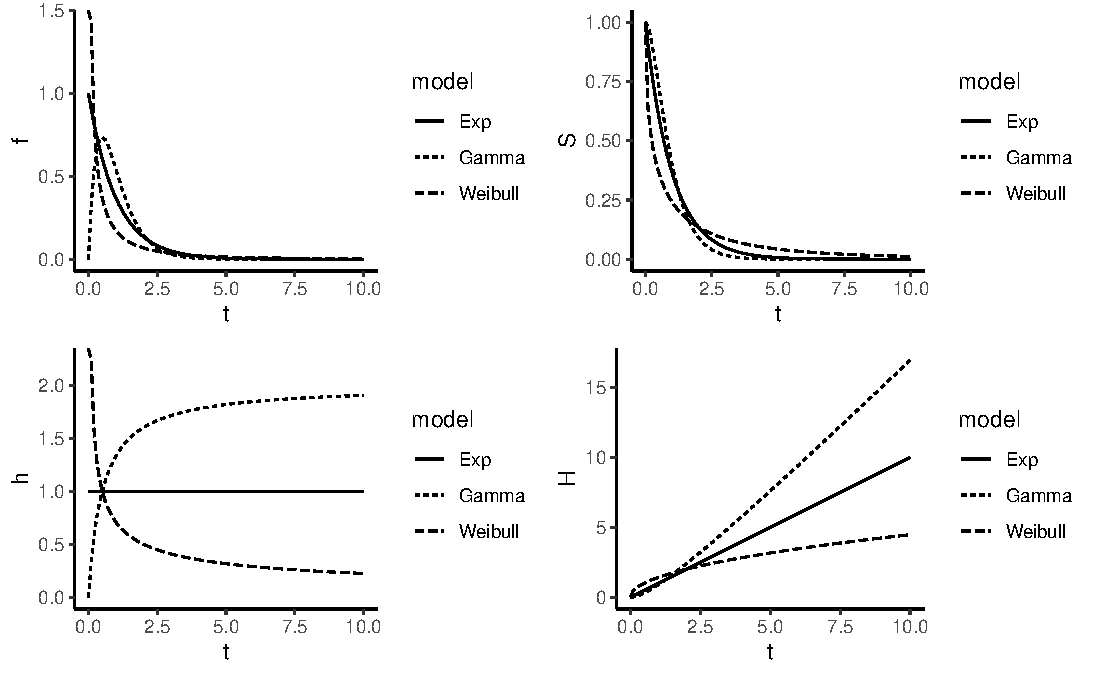
\includegraphics[width = \textwidth]{../figures/d_S_h_H_parametric}
\caption{Fonction de densité, de survie, de hasard et de hasard cumulée des modèles $\ExpDist(\beta = 1)$, $\GammaDist(\alpha = 2, \beta = 1/2)$ et $\WeibullDist(\alpha = 1 / 2, \beta = 1/2)$.}
\label{fig:d_S_h_H_parametric}
\end{figure}
L'approche paramétrique consiste à calibrer
plusieurs modèles puis à choisir le plus adapté grâce à des critère d'information.
\subsection{Critère d'information}
Les critères d'informations mesurent l'ajustement du modèle aux données. Ils sont basés sur la vraisemblance et pénalisent la compléxité du modèle (c'est à dire le nombre de paramètres). L'\textit{Akaike Information Criterion} (AIC) est défini par 
$$
\text{AIC} = 2k - 2 l(\Data;\hat{\theta}),
$$
où $k$ désigne le nombre de paramètre du modèle, voir \citet{Akaike1998}. Le Bayesian Information Criteria (BIC) est défini par 
$$
\text{BIC} = k\ln(n) - 2 l(\Data;\hat{\theta}),
$$
où $n$ désigne la taille de l'échantillon voir \citet{Schwarz1978}. le meilleur modèle est caractérisé par la plus petite valeur d'AIC et de BIC. le terme $- 2 l(\Data;\hat{\theta})$ correspond à la déviance du modèle par rapport au modèle qui aurait généré les données. 
\subsection{Test d'adéquation}
Une validation des modèles peut s'effectuer via des test d'adéquation statitique. Les hypothèses du test sont 
$$
\begin{cases}
H_0&\Prob(T\leq t)  = F(t; \theta)\\
H_1&\Prob(T\leq t)  \neq F(t; \theta)
\end{cases}
$$
les statistique de test sont définie par des écarts entre la fonction de répartition du modèle considéré $F(\cdot ; \hat{\theta})$ et la fonction de répartition empirique 
$$
F_n(t) = \frac{1}{n}\sum_{i=1}^n\ind_{t_i\leq t}.
$$
Le test de Kolmogorov-Smirnov s'appuie sur la distance 
$$
D_n = \underset{t\geq 0}{\sup}|F_n(t) - F(t; \theta)|,
$$
estimée concretement par 
$$
D_n=\max(D_-,D_+)
$$
où
$$
D_- =\underset{i = 1,\ldots n}{\max} i/n -F\left(t_{(i)}; \theta\right),\text{ et }D_- =\underset{i = 1,\ldots n}{\max} F\left(t_{(i+1)}; \theta\right) - i/n.
$$ 
On a le résultat de convergence suivant 
\begin{equation}\label{eq:convergence_ks}
\sqrt{n}D_n\overset{}{\rightarrow} K\text{ en loi,}
\end{equation}
où $K$ est une \va de loi de Kolmogorov. La fonction de répartition n'a pas une forme explicite mais cette distribution a été tabulé et encodé dans les logiciel statistiques. Soit $K_{1-\alpha}$ tel que 
$$
\Prob(K>K_{1-\alpha}) = \alpha.
$$ 
On rejette l'hypothèse $H_0$ si 
$$
\sqrt{n}D_n >K_{1-\alpha}.
$$
\begin{definition}
\begin{enumerate}
	\item $\alpha$ est le niveau du test, c'est à dire la probabilité de rejeter l'hypothèse nulle alors qu'elle est vraie
	$$
	\Prob(\sqrt{n}D_n>K_{1-\alpha}|H_0)
	$$
	\item La puissance du test, est la probabilité de rejeter l'hypothèse nulle alors qu'elle est fausse, soit 
	$$
	\beta = \Prob(\sqrt{n}D_n >  K_{1-\alpha}|H_1)
	$$
	\item La p-value est définie par  
	$$
	\text{p-value} = \Prob(K > \sqrt{n}D_n),
	$$
	On rejette l'hypothèse nulle au niveau $5\%$ si $\text{p-value} \leq 0.05$.
\end{enumerate}
\end{definition}
\begin{remark}
Le résultat de convergence \eqref{eq:convergence_ks} n'est pas valide lorsque les paramètre de la distribution doivent être estimés. Des méthodes de Monte Carlo de type bootstrap paramétrique doivent être mis en oeuvre pour déterminé la valeur critique du test (le $K_{1-\alpha}$).
\end{remark}






% !TEX root = ../main_lecture_notes.tex
\chapter{Approche non paramétrique}\label{chap:nonparametric}
Soit $T$ une variable aléatoire positive et un échantillon $t_1,\ldots, t_n$ de réalisations \iid de $T$. L'estimateur naturelle de la fonction de survie de $T$ est donnée par 
\begin{equation}\label{eq:fonction_survie_empirique}
\widehat{S}_n(t) =\frac{1}{n}\sum_{k=1}^n\ind_{t_k >t}.
\end{equation}
La loi des grands nombre indique qu'il s'agit d'un estimateur convergent de la fonction de survie. Dans une analyse de survie, nous devons prendre en compte le phénomène de censure. Pour chaque observation $k=1,\ldots, n$, nous observons 
$$
\Data = (x_k, \delta_k) = \left(t_k\land c_k, \ind_{t_k<c_k}\right),
$$
où $(c_k)_{k\geq1}$ est une suite de réels positives. Nous savons si l'observation est censurée via $\delta_k$, auquel cas la valeur censurée $c_k$ remplace la réalisation $t_k$. L'utilisation des $x_k$ brutalement dans l'estimateur \eqref{eq:fonction_survie_empirique} biaise l'estimation. Une alternative qui exploite mieux l'information disponible est l'estimateur de Kaplan-Meier.
\section{Estimateur de Kaplan-Meier et Nelson-Aalen}

Ce problème de valeurs observées censurées a été contournée par \citet{Kaplan1958} qui ont proposé un estimateur "produit-limite". Supposons que $T$ soit discrète à valeur dans $\{v_0,v_1,\ldots,\}$ tel que $0=v_0<v_1<\ldots$. Notons 
$$
h_0 =\Prob(T=v_0)\text{, et } h_k=\Prob(T=v_k|T> v_{k-1})\text{ pour } k\geq 1.
$$
\begin{remark}
Si $T$ est un \va continu alors on peu discrétiser la loi de $T$ en approchant $T$ par $h\lfloor T/h\rfloor$. Comme $h\lfloor T/h\rfloor\rightarrow T$ lorsque $h\rightarrow 0$ et l'approximation est d'autant meilleur que le pas de discrétisation $h$ est petit. 
\end{remark}
\begin{theo}
L'estimateur de Kaplan-Meier est donnée par 
\begin{equation}\label{eq:estimateur_KP}
\widehat{S_n}^{\text{KP}}(t) = \prod_{k: v_k\leq t}\left[1-\frac{d(v_k)}{n(v_k)}\right],
\end{equation}
où $d(v_k) = \sum_{i = 1}^n\delta_i\ind_{x_i\in [v_k,v_{k+1})}$ et $n(v_k) = \sum_{i = 1}^n\ind_{x_i\geq v_k}$. 
\end{theo}
\begin{remark}
Pour une \va T continue et un pas de discrétisation petit, on a 
$$
d(v_k) = d(t_k) = 1\text{ pour }k = 1,\ldots, n.
$$
\end{remark}
\begin{proof}
Nous allons considérer que les $h_k$ sont les paramètres du modèle, la vraisemblance des données s'écrit 
$$
\mathcal{L}(\Data;\theta) = \prod_{i=1}^n f(x_i; \theta)^{\delta_i}S(x_i;\theta)^{1-\delta_i},
$$
où $\Data = (x_i,\delta_i),\text{ }i = 1,\ldots, n$ et $\theta = h_0, h_1,\ldots$. Dans le cadre de notre modèle discret nous avons
$$
\mathcal{L}(\Data;\theta) = \prod_{i=1}^n \prod_{k=0}^\infty \left[p_k^{\ind_{x_i\in\left[v_k,v_{k+1}\right)}}\right]^{\delta_i}
\left[S_k^{\ind_{x_i\in[v_k,v_{k+1})}}\right]^{1-\delta_i},
$$
où
$$
p_k = \Prob(T = v_k)\text{, et }S_k = \Prob(T > v_k).
$$
On a 
$$
p_k = h_k S_{k-1}\text{ et }S_k = \prod_{j = 0}^k(1-h_j).
$$
On peut ré-écrire la vraisemblance
\begin{eqnarray*}
\mathcal{L}(\Data;\theta) &=& \prod_{i=1}^n \prod_{k=0}^\infty h_k^{\ind_{x_i\in\left[v_k,v_{k+1}\right)}\delta_i}\left[\prod_{j=0}^{k-1}(1-h_j)\right]^{\ind_{x_i\in\left[v_k,v_{k+1}\right)}\delta_i}
\left[\prod_{j=0}^{k}(1-h_j)\right]^{\ind_{x_i\in[v_k,v_{k+1})}(1-\delta_i)}\\
&=& \prod_{i=1}^n \prod_{k=0}^\infty h_k^{\ind_{x_i\in\left[v_k,v_{k+1}\right)}\delta_i}(1-h_k)^{-\ind_{x_i\in\left[v_k,v_{k+1}\right)}\delta_i}
\left[\prod_{j=0}^{k}(1-h_j)\right]^{\ind_{x_i\in[v_k,v_{k+1})}}\\
&=& \prod_{k=0}^\infty h_k^{d(v_k)}(1-h_k)^{-d(v_k)}\left[\prod_{j=0}^{k}(1-h_j)\right]^{\sum_{i = 1}^n\ind_{x_i\in[v_k,v_{k+1})}}
\end{eqnarray*}
On passe au log pour obtenir 
\begin{eqnarray*}
l(\Data;\theta) &=& \log\mathcal{L}(\Data;\theta)\\
&=& \sum_{k=0}^\infty \left\{d(v_k)\log(h_k)-d(v_k)\log(1-h_k) + \left[\sum_{j=0}^{k}\sum_{i = 1}^n\ind_{x_i\in[v_k,v_{k+1})}\log(1-h_j)\right]\right\}\\
&=&\sum_{k=0}^\infty \left\{d(v_k)\log(h_k)-d(v_k)\log(1-h_k)\right\} + \sum_{k=0}^\infty\left[\sum_{j=0}^{k}\sum_{i = 1}^n\ind_{x_i\in[v_k,v_{k+1})}\log(1-h_j)\right]\\
&=&\sum_{k=0}^\infty \left\{d(v_k)\log(h_k)-d(v_k)\log(1-h_k)\right\} + \sum_{j=0}^\infty\left[\sum_{k=j}^{\infty}\sum_{i = 1}^n\ind_{x_i\in[v_k,v_{k+1})}\log(1-h_j)\right]\\
&=&\sum_{k=0}^\infty \left\{d(v_k)\log(h_k)-d(v_k)\log(1-h_k)\right\} + \sum_{j=0}^\infty\log(1-h_j)\sum_{i = 1}^n\sum_{k=j}^{\infty}\ind_{x_i\in[v_k,v_{k+1})}\\
&=&\sum_{k=0}^\infty \left\{d(v_k)\log(h_k)-d(v_k)\log(1-h_k)\right\} + \sum_{j=0}^\infty\log(1-h_j)\sum_{i = 1}^n\sum_{k=j}^{\infty}\ind_{x_i\in[v_k,v_{k+1})}\\
&=&\sum_{k=0}^\infty \left\{d(v_k)\log(h_k)-d(v_k)\log(1-h_k)\right\} + \sum_{j=0}^\infty\log(1-h_j)\sum_{i = 1}^n\ind_{x_i\geq v_j}\\
&=&\sum_{k=0}^\infty \left\{d(v_k)\log(h_k)-d(v_k)\log(1-h_k)\right\} + \sum_{j=0}^\infty\log(1-h_j)n(v_j)\\
&=&\sum_{k=0}^\infty d(v_k)\log(h_k)-[n(v_k) - d(v_k)]\log(1-h_k).\\
\end{eqnarray*}
On recherche les $h_k$ qui maximisent la log vraisemblance, c'est à dire solution de
$$
\frac{\partial}{\partial h_k}l(\Data;\theta) = 0\Leftrightarrow \frac{d(v_k)}{h_k}-\frac{n(v_k)-d(v_k)}{1-h_k}=0.
$$
On en déduit que
$$
\widehat{h}_k = \frac{d(v_k)}{n(v_k)}.
$$
On vérifie également que 
$$
\frac{\partial^2 l}{\partial h_k\partial h_l} (\Data;\theta)=\begin{cases}
0,&\text{ si }l\neq k\\
-\frac{d(v_k)}{h_k^2}-\frac{n(v_k)-d(v_k)}{(1-h_k)^2},&\text{ sinon.}

\end{cases}
$$
La matrice Hessienne est définie négative. On approche la fonction de survie par 
$$
S(t)\approx S_k,\text{pour }t\in [v_k,v_{k+1}),
$$
puis on estime par 
$$
\widehat{S}_n(t)=\prod_{k:v_k\leq t}\left[1-\frac{d(v_k)}{n(v_k)}\right].
$$
\end{proof}
Pour proposer un estimateur de la fonction de hasard cumulée, on pourrait s'appuyer sur la relation entre la fonction de hasard cumulé et la fonction de survie
$$
\widehat{H}^{\text{KP}}_n(t) = -\ln\left[\widehat{S}^{\text{KP}}_n(t)\right] = -\sum_{k:v_k\leq t}\ln\left[1-\frac{d(v_k)}{n(v_k)}\right].
$$
L'estimateur de Nelson-Aalen (\citet{Nelson1972} et \citet{Aalen1978}) est un estimateur de la fonction de hasard cumulé qui se base sur l'estimation des taux de hasard instantanée.
\begin{coro}
$$
\widehat{H}_n^{\text{NA}}(t) = \sum_{k:v_k\leq t}\frac{d(v_k)}{n(v_k)}.
$$
\end{coro}
\begin{proof}
Pour une \va $T$ discrète à valeur dans $\{v_0, v_1,\ldots\}$, on a 
$$
H(t) = \sum_{k:v_k\leq t} h_k.
$$
On remplace les $h_k$ par leur contre-partie empirique $\widehat{h}_k = d(v_k)/n(v_k)$ déterminé précédemment.
\end{proof}
\begin{remark}
Pour $d(v_k)/n(v_k)$ suffisament petit, on a 
$$
\ln\left[1-\frac{d(v_k)}{n(v_k)}\right]\approx -d(v_k)/n(v_k),
$$ 
et 
$$\widehat{H}_n^{\text{NA}}(t)\approx \widehat{H}_n^{\text{KP}}(t).$$
\end{remark}

\section{Variance et intervalle de confiance}
\subsection{Rappel des propriétés de l'estimateur du maximum de vraisemblance}
Soit $\Data = (x_1,\ldots, x_n)$ un échantillon \iid de réalisations de $X$ \va de densité $f(x;\theta)$. On note $l(\Data ; \theta)$ la log-vraisemblance du modèle et $\widehat{\theta} =(\widehat{\theta}_1,\ldots, \widehat{\theta}_k) $ l'estimateur du maximum de vraisemblance.
% \begin{definition}\label{def:score_info_fisher}
% la fonction de score est définie par 
% $$
% s(X;\theta) = \frac{\partial}{\partial\theta}\ln f(X;\theta).
% $$
% L'information de Fisher de l'échantillon $(x_1,\ldots, x_n)$ est définie par
% $$
% I_n(\theta) = \V\left[\sum_{i=1}^n s(x_i;\theta)\right] = \sum_{i=1}^n \V\left[s(x_i;\theta)\right]
% $$
% \end{definition}
% On note que 
% $$
% \E\left[s(X;\theta)\right] = 0
% $$
% et donc
% $$
% \V\left[s(x_i;\theta)\right] = \E\left[s(x_i;\theta)^2\right]
% $$
% L'estimateur du maximum de vraisemblance $\widehat{\theta}$ annule l'approximation de Monte Carlo de la moyenne du score. 
% \begin{prop}
% Sous certaine conditions de régularité, on a 
% $$
% I_n(\theta) = nI(\theta),  
% $$
% avec 
% $$
% I(\theta) = -\E\left(\frac{\partial^2}{\partial\theta^2}\ln f(X;\theta)\right).
% $$
% \end{prop}
\begin{theo}
Sous certaines conditions de régularité, on a
$$
\widehat{\theta}\sim \NormalDist\left(\theta,I_n(\widehat{\theta})^{-1}\right),\text{ pour } n\rightarrow\infty,
$$
où 
$$
I_n(\widehat{\theta})^{-1} =  \left(-\frac{\partial^2}{\partial\theta^2}l(\Data;\widehat{\theta})\right)^{-1},
$$
est la matrice d'information de Fisher. De plus, 
$$
\widehat{\theta}_j\sim\NormalDist(\theta_j, I_n(\widehat{\theta})^{-1}(j,j)),
$$
où $I_n(\widehat{\theta})^{-1}(j,j)$ est le $j^{\text{ème}}$ terme diagonale de la matrice $I_n(\widehat{\theta})^{-1}$. A noter que le terme $I_n(\widehat{\theta})^{-1}(i,j)$ correspond à la covariance entre $\widehat{\theta}_i$ et $\widehat{\theta}_j$.
\end{theo}
L'estimateur du maximum de vraisemblance est asymptotiquement normal ce qui permet de construire des intervalles de confiance et d'approcher sa matrice de variance-covariance par
$$
\V\left(\widehat{\theta}\right) = I_n(\widehat{\theta})^{-1}.
$$
Une transformation régulière de l'estimateur du maximum de vraisemblance est aussi asymptotiquement normal.
\begin{prop}
Soit $\widehat{\theta}$ l'estimateur du maximum de vraisemblance de $\theta$ et $g$ une fonction dérivable, on note $^t\nabla g(\theta) = \left(\frac{\partial g}{\partial \theta_1}(\theta),\ldots, \frac{\partial g}{\partial \theta_k}(\theta)\right)$   alors 
$$
g(\widehat{\theta})\sim\NormalDist\left(g(\theta), \,^t\nabla g\left(\widehat{\theta}\right)I_n(\widehat{\theta})^{-1}\nabla g\left(\widehat{\theta}\right)\right).
$$
\end{prop}
Ce résultat est connu sous le nom de méthode delta. Pour plus de détails sur ces résultats voir par exemple \cite[Chapitre 9]{Wasserman2013}.
\subsection{Application à l'estimateur de Kaplan-Meier}
On a $\theta= (h_0,h_1,\ldots)$ et
\begin{equation}\label{eq:partial_derivative_log_like}
\frac{\partial^2 }{\partial h_k\partial h_l} l(\Data;\theta)=\begin{cases}
0,&\text{ si }l\neq k\\
-\frac{d(v_k)}{h_k^2}-\frac{n(v_k)-d(v_k)}{(1-h_k)^2},&\text{ sinon.}
\end{cases}
\end{equation}
La matrice d'information de Fisher est diagonale, ce qui implique une indépendance asymptotique des $\widehat{h}_{k}$. En substituant $h_k$ par $\widehat{h}_k = d(v_k)/n(v_k)$, on obtient 
$$
\V(\widehat{h}_k)\rightarrow \frac{d(v_k)[n(v_k)-d(v_k)]}{n(v_k)^3},\text{ pour }n\rightarrow \infty.
$$
L'estimateur de Kaplan-Meier vérifie
$$
\ln\widehat{S}_n(t)=\sum_{k:v_k\leq t}\ln\left[1-\widehat{h}_k\right].
$$
On applique la méthode delta avec la fonction $g:x\mapsto \ln(1-x)$. On a 
$$
g(\widehat{h}_k) - g(h_k)\sim \NormalDist(0,\V(\widehat{h}_k)g'(\widehat{h}_k)^2
).
$$
On en déduit que 
$$
\V\left[\ln(1-\widehat{h}_k)\right]\rightarrow \frac{d(v_k)}{n(v_k)[n(v_k) - d(v_k)]},\text{ lorsque }n\rightarrow\infty.
$$
L'estimateur de Kaplan Meier vérifie
$$
\ln\widehat{S}_n(t)\sim\NormalDist[\ln S(t), \V\ln\widehat{S}_n(t)]
$$
où
$$
\V\ln\widehat{S}_n(t)\rightarrow \sum_{k:v_k\leq t}\frac{d(v_k)}{n(v_k)[n(v_k) - d(v_k)]}\text{ pour }n\rightarrow\infty,
$$
car les $\widehat{h}_k$ sont asymptotiquement indépendants. On applique une deuxième fois la méthode delta sur $\ln\widehat{S}_n(t)$ avec $g:x\mapsto \e^x$ pour aboutir à 
$$
\widehat{S}_n(t) - S(t)\sim \NormalDist\left(0,\widehat{S}_n(t)^2\V\ln\widehat{S}_n(t)
\right).
$$
L'estimateur de la variance $\widehat{S}_n(t)^2\V\ln\widehat{S}_n(t)$ de l'estimateur de Kaplan-Meier est parfois appelé estimateur de Greenwood.
% \section{Troncature à gauche et censure à droite}
% Dans le cadre d'applications actuarielles, on rencontre souvent des données tronquées à gauche et censurée à droite. Les observations sont
% \begin{itemize}
% \item $\tau_i$ instant à partir duquel l'évènement $i$ peut être observé. 
% \item $x_i = t_i\land c_i$ et $\delta_i = \ind_{t_i\leq c_i}$ si $x_i>\tau_i$ et $\emptyset$ sinon.
% \end{itemize}
% \begin{ex}
% Dans le cadre d'un portefeuille d'assurance prévoyance pour lequel on souhaite établir une loi de maintien en incapacité, si l'entrée en incapacité se produit avant l'entrée en portefeuille alors nous avons pas accès à la durée de l'état d'incapacité.
% \end{ex}
% La prise en compte de la troncature à droite se fait en adaptant les décomptes d'observations avec 
% $$
% d(v_k) = \sum_{i = 1}^n\delta_i\ind_{x_i\in [v_k,v_{k+1})}\ind_{x_i> \tau_i}\text{, et }n(v_k) = \sum_{i = 1}^n\ind_{x_i\geq v_k}\ind_{x_i> \tau_i}.
% $$
% A noter que l'estimateur de Kaplan-Meier estime la fonction de survie de $T$ sachant que $T>\underset{i=1,\ldots,n}{\min}(\tau_i).$
\section{Comparaison de la courbe de survie dans deux populations}
L'objectif est de tester statistiquement l'égalité des taux de hasard instantanées au sein de deux populations. Sous $(H_0)$, on $h_k^1 =h_k^2$ pour tout $k$. On définit 
$$
d_j(v_k),\text{ et } n_j(v_k)\text{ pour }j=1,2. 
$$
les décomptes d'évènement au sein des groupes $1$ et $2$. Sous $H_0$, $d_j(v_k)$ suit une loi hypergéométrique $\text{H}-\GeometricDist[n(v_k), n_j(v_k),  d(v_k)]$.
\begin{definition}
Une urne contient $N$ boules dont $K$ boules blanches et $N-K$ boules noires. On réalise $h$ tirage aléatoire sans remise dans cette urne et on note $X$ le nombre de boules blanches tirées. La \va $X\sim \text{H}-\GeometricDist(N, K, h)$ admet une loi de probabilité donnée par
$$
\Prob(X = x)=\frac{\binom{K}{x}\binom{N-K}{h-x}}{\binom{N}{h}},\text{ pour }\max(0, h-(N-K))\leq x\leq\min(K,h).
$$ 
Les moyenne et variance ont données par 
$$
\E(X) =h\frac{K}{N},\text{ et }\V(X) = h\frac{K}{N}\frac{N-K}{N}\frac{N-h}{N-1}.
$$
\end{definition}
La statistique du log-rang compare la valeur observée $O_{j,k} = d_j(v_k)$ à la valeur attendue $E_{j,k} = d(v_k)\frac{n_j(v_k)}{n(v_k)}$ sous $H_0$ avec 
\begin{equation}\label{eq:log_rank_stat}
Z_j=\sum_{k: d(v_k)\geq 1}\frac{(O_{j,k} - E_{j,k})}{\sqrt{\sum_{k: d(v_k)\geq 1}V_{j,k}}}\sim \NormalDist(0,1),\text{ pour }j = 1,2,
\end{equation}
où
$$
V_{j,k}=d(v_k)\frac{n_j(v_k)}{n(v_k)}\frac{n(v_k)-n_j(v_k)}{n(v_k)}\frac{n(v_k)-d(v_k)}{n(v_k)-1}.
$$
La convergence \eqref{eq:log_rank_stat} est une application du théorème centrale limite\footnote{une généralisation du TCL de Lyapunov ou Lindeberg-Feller, voir \url{https://en.wikipedia.org/wiki/Central_limit_theorem}}, d'autant plus valide que $\#\{k: d(v_k)\geq 1\}$ est grand. Un autre test du log-rang consiste à élever la statistique de test au carré et alors $Z_j^2\sim \chi^2(1)$. Une meilleure approximation de la distribution asymptotique de la statistique de test a été obtenu par \citet{Peto1972}. On peut également pondérer les observation en ajoutant des poids $w_j$ avec 
\begin{equation}\label{eq:log_rank_stat_weighted}
Z_j=\sum_{k: d(v_k)\geq 1}w_j\frac{(O_{j,k} - E_{j,k})}{\sqrt{\sum_{k: d(v_k)\geq 1}w_j^2V_{j,k}}}\sim \NormalDist(0,1),\text{ pour }j = 1,2.
\end{equation}


% !TEX root = ../main_lecture_notes.tex
\chapter{Modèles à hasard proportionel}\label{chap:Ph_models}
Nous étudions des données $t_1,\ldots, t_n$ censurés à droite 
$$
(x_i,\delta_i) = \left(t_i\land c_i,\ind_{t_i\leq c_i}\right),\text{  }i=1,\ldots, n.
$$
Chaque évènement $i$ est associé à des caractéristiques ou variable explicatives 
$$
z_{i1},\ldots, z_{ip}\text{ }i=1,\ldots, n.
$$
L'objectif est d'étudier la loi conditionelle de la durée $T$ sachant $Z$.
\section{Définition du modèle}
Le modèle à hasard proportionel spécifie la fonction de hasard par 
\begin{equation}\label{eq:cox_proportional_hazard}
h(t; z, \beta) = h_0(t)\e^{z \beta}=h_0(t)\e^{z_1\beta_1+\ldots+z_p\beta_p},
\end{equation}
où la fonction $h_0$ est le risque de base, modifié par les caractéristiques individuelles suivant les coefficients de regressions $\beta = (\beta_1\text{ \ldots }\beta_p)$. L'impact multiplicatif des variables sur le taux de hasard explique le nom du modèle.
\begin{ex}
	\begin{enumerate}
		\item Prenons l'exemple d'un modèle ne comprenant qu'une variable explicative $Z\in\{0,1\}$ alors le risque instantané s'écrit 
		$$
		h(t)=\begin{cases}
		h_0(t),&\text{ si }Z_0 = 0\\
		h_0(t)\e^{\beta},&\text{ sinon}.
		\end{cases}
		$$
		Le risque est multiplié par $\e^\beta$ lorsque $Z_1=1$. Le signe de $\beta$ indique si le risque augmente $\beta>0$ ou diminue $\beta>0$
		\item pour une variable continue $Z\in \RL$, le coefficient de regression donne l'impact d'une variation d'amplitude $1$. En effet, 
		$$
\frac{h_0(t)\e^{\beta\cdot (z+1)}}{h_0(t)\e^{\beta\cdot z}} = \e^{\beta}.
		$$
	\end{enumerate}
\end{ex}
\section{Inférence des paramètres}
La vraisemblance du modèle pour les données $\Data = (x_k,\delta_k)_{k=1,\ldots, n}$ s'écrit 
\begin{equation}\label{eq:likelihood_cox}
\mathcal{L}(\Data;\theta) =\prod_{i=1}^n \left[h_0(x_i)\e^{z_i\cdot \beta}\right]^{\delta_i}\cdot\exp\left(-\e^{z_i\cdot\beta} \int_0^{x_i}h_0(s)\text{d}s\right) ,
\end{equation}
où $\theta = (h_0,\beta)$. Il n'est pas possible d'inférer les paramètres avec la vraisemblance \eqref{eq:likelihood_cox} sans donner une structure au risque de base. 
\begin{remark}
Le modèle \eqref{eq:cox_proportional_hazard} est le modèle de \citet{Cox1972}. L'étude se focalise plus sur l'impact des covariable $Z_1,\ldots, Z_p$ que sur le risque de base $h_0$ qui peut prendre une forme arbitraire. \citet{Cox1972} défini une vraisemblance partielle qui correspond à la probabilité que les évènements se produisent dans l'ordre observé. Nous souhaitons également estimé le risque de base, nous allons donc supposer que $h_0$ est une fonction continue par morceaux, voir \citet{Breslow1975}.
\end{remark}
Soit 
$$
0=v_0<v_1<v_2<\ldots<v_K<v_{K+1}=\infty,
$$
tels que $v_1,\ldots, v_K$ correspondent aux observations ordonnées, distinctes et non censuré. Le risque de base est donnée par
$$
h_0(t)=\sum_{k=1}^{K}\alpha_k\ind_{(v_{k-1}, v_{k}]}(t),t\geq 0.
$$
Les paramètres du modèle sont données par $\theta = (\alpha, \beta)$. La log vraisemblance s'écrit
\begin{eqnarray*}
l(\Data;\theta)&=&\sum_{i=1}^n\delta_i\{\log[h_0(x_i)]+z_i\beta\}-\e^{z_i\beta}\int_0^{x_i}h_0(s)\text{d}s\\
&=& \sum_{i=1}^n\delta_i\sum_{k=1}^K\left[\log(\alpha_k)+\delta_i z_i\beta\right]\ind_{x_i = v_k} -\e^{z_i\beta}\sum_{k=1}^K\alpha_k\int_0^{x_i}\ind_{(v_{k-1}, v_k]}(s)\text{d}s\\
&=& \sum_{k=1}^K\log(\alpha_k)d(v_k)+s_k\beta -\alpha_k\sum_{i=1}^{n}\int_0^{x_i}\e^{z_i\beta}\ind_{(v_{k-1}, v_k]}(s)\text{d}s\\
&=& \sum_{k=1}^K\log(\alpha_k)d(v_k)+s_k\beta -\alpha_k\left\{\sum_{i=1}^{n}\e^{z_i\beta}\left[(v_k - v_{k-1})\ind_{x_i\geq v_k} +(x_i - v_{k-1})\ind_{(v_{k-1},v_k]}(x_i)\right]\right\}\\
&=& \sum_{k=1}^K\log(\alpha_k)d(v_k)+s_k\beta -\alpha_kE_k(\beta),\\
\end{eqnarray*}
où $d(v_k)$ est le nombre d'évènements se produisant exactement à l'instant $v_k$ et $s_k$ la somme des caractéristiques ($\sum_i \delta_i z_i$) de ces évènements. L'estimateur du maximum de vraisemblance $\widehat{\theta}$ est obtenu en annulant les dérivées premières, il vient 
$$
\widetilde{\alpha}_k = \frac{d(v_k)}{E_k(\beta)}, 
$$
où 
$$
E_k(\beta) = \sum_{i=1}^{n}\e^{z_i\beta}\left[(v_k - v_{k-1})\ind_{x_i\geq v_k} +(x_i - v_{k-1})\ind_{(v_{k-1},v_k]}(x_i)\right],
$$ 
est l'exposition.
\begin{remark}
Dans le papier original de \citet{Breslow1975}, les données censurés entre $v_{k-1}$ et $v_k$ sont remplacées par $v_{k-1}$ (l'observation non censuré la plus proche). Cela simplifie l'exposition qui devient 
$$
E_k(\beta) = \sum_{i=1}^{n}\e^{z_i\beta}(v_k - v_{k-1})\ind_{x_i\geq v_k}.
$$
\end{remark}
On recherche $\beta$ qui annule
$$
\frac{\partial}{\partial \beta}l[\Data; (\widetilde{\alpha},\beta) ] = \sum_{k=1}^K s_k - d(v_k)\frac{E_k'(\beta)}{E_k(\beta)}.
$$
Le programme d'optimisation alterne les mises à jour des $\tilde{\alpha}$ et $\beta$ (numériquement pour $\beta$). Les estimateur de $\alpha$ et $\beta$ sont convergent et asymptotiquement normaux puisque issu du maximum de vraisemblance, la matrice de variance-covariance est donnée par la matrice Hessienne de la log vraisemblance
$$
I_n(\theta) = \left[-\frac{\partial^2}{\partial\theta^2}l\left(\Data;\widehat{\theta}\right)\right].
$$ La fonction de hasard cumulée de base est estimée par 
$$
\widehat{H}_0(t) = \sum_{k=1}^K\frac{d(v_k)}{E_k(\widehat{\beta})}\ind_{v_k\leq t}.
$$
Il est possible d'obtenir une loi asymptotique pour cette estimateur, voir \citet{Spiekerman1998}, afin de construire des intervalles de confiance.
\section{Test d'hypothèse}
\subsection{Significativité des coefficients: le test de Wald}
Pour un paramètre univarié $\theta$ dont l'estimateur $\widehat{\theta}$est asymptotiquement normal. On peut effectuer une test de Wald pour tester sa nullité
$$
(H_0): \theta =0\text{  }(H_1):\theta\neq 0.
$$
La statistique de test est donnée par
$$
\frac{\widehat{\theta}}{\widehat{\text se}}\sim\NormalDist(0,1),
$$ 
où $\widehat{\text se}$ est une estimation de l'écart-type type de $\widehat{\theta}.$ Ici la racine carré du coefficient diagonal correspondant de l'inverse de la matrice de Fisher.
\subsection{Significativité du modèle: le test du rapport de vraisemblance}
Le test du rapport de vraisemblance test des hypothèses du type
$$
(H_0): \theta\in \Theta_0.\text{  }(H_1):\theta \notin\Theta_0,
$$
où $\Theta_0$ est une restriction de l'espace des paramètres $\Theta$, avec $\Theta_0\subset \Theta$. La statistique du test corrrespond est un ratio de log vraisemblance donnée par 
$$
\lambda = 2\log\frac{\underset{\theta \in \Theta}{\sup}\mathcal{L}\left(\Data ; \theta\right)}{\underset{\theta \in \Theta_0}{\sup}\mathcal{L}\left(\Data ; \theta\right)}.
$$
L'ensemble $\Theta_0$ consiste souvent en l'ensemble $\Theta$ pour lequel certain paramètre sont fixés. Supposons que $\theta = (\theta_1,\ldots,\theta_p)$ et que l'on souhaite tester l'hypothèse
$$
(H_0):\theta\in \Theta_0= \{\theta : \theta_1 = \theta_1^0,\ldots,\theta_q = \theta^0_q\},\text{ tel que } q \leq p, 
$$
alors 
$$
\lambda \sim \chi^2_{q}.
$$
La significativité du modèle de Cox test l'hypothèse de nullité simultanée de tout les coefficients. Concrètement 
$$
(H_0): \beta_1=0,\ldots\beta_p = 0\text{ }(H_1):\beta_1\neq0,\ldots\beta_p \neq 0,
$$
et $\lambda \sim \chi_p^2$.
\subsection{Vérification de l'hypothèse de proportionalité}
Dans le cadre du modèle de Cox, on s'intéresse à la loi jointe du couple $(T,Z)$. Supposons que $Z$ soit un vecteur aléatoire sur un espace d'état discret $E$ et $T$ soit également une \va discrète. Le modèle de Cox donne la fonction de hasard de la durée $T$ sachant le vecteur de covariable $Z$, c'est à dire 
$$
\Prob(T = t|Z =z,T\geq t) = h(t|z) = h_0(t)\e^{z\beta}.
$$
La loi de $Z|T=t$ est obtenue par 
\begin{eqnarray*}
\Prob(Z=z|T=t) &=& \frac{\Prob(Z=z,T=t)}{\Prob(T=t)}\\
&=&\frac{\Prob(Z=z,T=t, T\geq t)}{\sum_{z\in E}\Prob(T=t, Z=z, T\geq t)} \\
&=& \frac{\Prob(T=t|Z=z,T\geq t)\Prob(Z=z,T\geq t)}{\sum_{z\in E}\Prob(T=t| Z=z, T\geq t)}\\
&=& \frac{h_0(t)\e^{z\beta}\Prob(Z=z,T\geq t)}{\sum_{z\in E}\Prob(T=t| Z=z, T\geq t)\Prob(Z=z, T\geq t)}\\
&=&\frac{\E(e^{\beta Z}\ind_{\{Z = z, T\geq t\}})}{\E(e^{\beta Z}\ind_{T\geq t})}
\end{eqnarray*}
En présence d'un échantillon \iid $(t_i, z_i)_{i = 1,\ldots, n}$, cette loi peut être estimée par 
$$
\widehat{\Prob}(Z=z|T=t) = \frac{\sum_{i = 1}^n\e^{\widehat{\beta} z_i}\ind_{\{ z_i = z, t_i\geq t\}}}{\sum_{i = 1}^n \e^{\widehat{\beta} z_i}\ind_{t_i\geq t}}.
$$
cette estimateur demeure valide en remplaçant les observation $t_i$ par les observations censurées à droite $x_i$. Soient $v_1<\ldots < v_K$ les temps d'occurence des évènements distincts et non censurés. On peut comparer les caractéristiques moyenne observée et attendu des évènement s'étant produit aux temps $v_k,k=1,\ldots, K$ en calculant la différence
$$
r_k = Z(v_k) - \E(Z|T = v_k) = \frac{\sum_{i=1}^nz_i\ind_{x_i = v_k}}{d(v_k)}  - \sum_{i = 1}^nz_i\frac{\e^{\widehat{\beta} z_i}\ind_{\{ x_i\geq v_k\}}}{\sum_{i = 1}^n \e^{\widehat{\beta} z_i}\ind_{x_i\geq v_k}}.
$$
Les $r_k$ sont appelés résidus de \citet{SCHOENFELD1982}. Nous allons tester l'hypothèse de proportionalité séparément pour chacune des variables explicatives, cela revient à considérer $Z$ et $\beta$ comme des scalaires. On définit une fonction de hasard alternative avec 
$$
h^{\text{alt}}(t|z) = h_0(t)\exp[z\beta(t)] = h_0(t)\exp[z(\widehat{\beta}+\gamma g(t)],
$$
pour $\gamma\in \RL$ et $g:\RL_+\rightarrow\RL$. On test la significativité du coefficient $\gamma$ avec 
$$
(\text{H}_0): \gamma = 0.
$$
Les résidus se ré-écrivent 
$$
r_k = Z(v_k) - \E^\text{alt}(Z|T = v_k) + [\E^\text{alt}(Z|T = v_k)-\E(Z|T = v_k)] = Z(v_k) - M(\widehat{\beta}(v_k), v_k) + [M(\widehat{\beta}(v_k), v_k)-M(\widehat{\beta}, v_k)]
$$
On effectue un développement limité de $M(\widehat{\beta}(v_k), v_k)$  au voisinage de $\widehat{\beta}$. Il vient 
$$
r_k = Z(v_k) - M(\widehat{\beta}(v_k), v_k) + V(\widehat{\beta}, v_k)\gamma g(v_k),
$$
où
$$
V(\widehat{\beta}, v_k) = \frac{\partial}{\partial x} M(x, v_k)\Big|_{x = \widehat{\beta}} \approx \E(Z^2|T = v_k) - \E(Z|T = v_k)^2.
$$
L'espérance sous $H_0$ des résidus standardisés $r_k^\ast  = r_k /V(\widehat{\beta}, v_k)$ vérifie 
$$
\E(r_k^\ast) = \gamma g(v_k).
$$
Cela suggère une relation linéaire entre les $r_k^\ast$ et les $g(v_k)$. On peut choisir pour $g$ une fonction arbitraire. Un choix commun est l'identité. La significativité du coefficient $\gamma$ est établi par un un test de student sur le coefficient $\gamma$ vu comme la pente de la regression linéaire entre les série $r_k^\ast$ et $g(t_k)$. La significativité de toutes les covariables simultanément est possible également, grâce aux travaux de \citet{GRAMBSCH1994}.



% !TEX root = ../main_lecture_notes.tex
\chapter{Table de mortalité}\label{chap:mortality_table}

En assurance-vie, les modèles de projections des cash-flows permettant d'évaluer les engagements de l'assureur repose sur l'utilisation de tables de mortalité. Il s'agit d'un tableau comprenant pour chaque âge $x$ la probabilité de décès avant d'atteindre l'âge $x+1$. Les probabilités de décès peuvent variées en fonction du genre des individus. la réglementation (Article A132-1 à A132-19 du codes des assurance\footnote{\url{https://www.legifrance.gouv.fr/codes/article_lc/LEGIARTI000035514715}}) impose l'utilisation de tables réglementaires TH et TF $00-02$ pour l'évaluation des engagements liées aux garanties décès. Les tables de mortalités peuvent inclure 
\begin{itemize}
\item l'année calendaire pour prendre en compte une situation particulière liée à une année (par exemple une pandémie mondiale)
\item l'année de naissance des individus (génération ou cohortes) pour capter l'allongement progressif de la durée de vie des individus. 
\end{itemize}
L'évaluation des engagements pour les garanties viagère se fait en utilisant des tables réglementaires par génération TGH et TGF $05$ qui fournissent une table de mortalité pour chaque année de naissance. Les assureurs peuvent aussi utiliser une table de mortalité d'expérience s'ils considèrent que le risque de mortalité pour leur portefeuille d'assurés diffère significativement du risque pour la population générale. Les probabilités de décès, la méthode de calculs et les données utilisées doivent être audité par un actuaire indépendant certifié. Les méthodes vues dans ce chapitre sont présentées dans le cadre de la mortalité mais peuvent s'appliquer dans d'autre contexte pour construire des lois de rachat, d'entrée en incapacité, en invalidité ou en dépendance, des lois de maintien en incapacité.
\section{Estimation des probabilités de décès et des taux de mortalité}\label{sec:mortality_rate}
\subsection{Notations et donées}\label{sssec:notation}
Soit $T$ la durée de vie d'un individu. Supposons que l'on dispose d'information sur un nombre $N$ d'individus
\begin{itemize}
  \item $\Data = \{t_i\}$: âge exacte de décès
  \item $\Data =\{x_i, \delta_i\}$: âge exacte de décès censuré
  \item $\Data = \{E^0_x,d_x\}$: nombre de survivant (initial) et nombre de décès à l'âge $x$
  \item $\Data = \{E^C_x,d_x\}$: nombre de survivant (central) et nombre de décès à l'âge $x$
\end{itemize}
Nous pouvons estimer la fonction de survie $\widehat{S}(t)$. Dans l'étude de la mortalité on s'intéresse à la durée de vie résiduelle à l'âge $x$ défini par 
$$
T_x\sim T-x|T>x.
$$
On s'intéresse au quantités présentées dans le \cref{tab:notation_mortality_table}
\begin{table*}[ht!]\centering
% \ra{1.3}
\begin{tabular}{@{}lllll@{}}
\toprule
$E_x^0$&&&&Exposition initiale\\
&&&&Nombre de survivant jusqu'à l'âge $x$\\
\midrule
$E_x^c$&&&$(E_x^0 + E_{x+1}^0)/2 $&Exposition centrale\\

&&&$\sum_{i=1}^N\tau_{x,i}$&Cumul des temps d'observation d'individu d'age $x$\\
\midrule

$d_x$&&&$E^0_{x} - E^0_{x+1}$&Nombre de décès à l'âge $x$\\
\midrule
$q_x$&$\Prob(T_x \leq 1)$&$\Prob(T \leq x+1|T> x)$&$d_x/E^0_x$& Probabilité de décès d'un individu d'âge $x$ \\
&&&$1-\e^{-d_x/E_x^c}$&avant d'atteindre l'âge $x+1$\\
\midrule
$p_x$&$\Prob(T_x > 1)$&$\Prob(T > x+1|T> x)$&$1-q_x$ &Probabilité de survie d'un individu d'âge $x$ \\
&&&&jusqu'à l'âge $x+1$\\
\midrule
$\,_tp_x$&$\Prob(T_x > t)$&$\Prob(T > x+t|T> x)$&$\prod_{s=1}^tp_{x+s}$& Probabilité de survie d'un individu d'âge $x$ \\
&&&&jusqu'à l'âge $x+t$\\
\midrule
$\,_tq_x$&$\Prob(T_x \leq t)$&$\Prob(T \leq x+t|T> x)$&$1 - \,_tp_x$& Probabilité de décès d'un individu d'âge $x$ \\
&&&&avant d'atteindre l'âge $x+t$\\
\midrule

$\mu_x$&\multicolumn{2}{c}{$\lim_{h\rightarrow 0}h^{-1}\Prob(T_x\in[x,x+h])$}&$-\log(p_x)$ &Taux de décès instantanée à l'âge $x$\\
\midrule
$e_x$&$\E(T_x)$&$\E(T-x|T>x)$&$\sum_{t\geq 0} \,_tp_x$ &Espérance de vie résiduelle à l'âge $x$\\
\bottomrule
\end{tabular}
\caption{Récapitulatif des notations des tables de mortalités}
\label{tab:notation_mortality_table}
\end{table*}
Les estimateurs des quantités d'intérêts $q_x, p_x$ et $\mu_x$ utilisent les expositions et les nombre de décès $d_x$. Leur justification est donnée dans la section suivante.
\subsection{Estimation}
La justification de l'expression des estimateurs du \cref{tab:notation_mortality_table} repose sur la maximisation de la vraisemblance des données. Les données de mortalités se limitent aux effectifs par âge $E^0_x$, avec $\Data = \{E^0_x\}_{x\in\mathbb{N}}$. Un extrait de la table réglementaire $TF 00-02$ est donné par \cref{tab:TF002}.
\begin{table}[ht!]
\centering
\begin{tabular}{ll}
  \hline
 Age & $l_x$ \\ 
  \hline
 $0$ & $100,000 $\\ 
 $1$ &$ 99,616 $\\ 
 $2$ &$ 99,583 $\\ 
 $3$ &$ 99,562 $\\ 
 $4$ &$ 99,545 $\\ 
 $\vdots$ &$\vdots $\\
 $111$ & $4$ \\ 
 $112$ & $1$ \\ 
   \hline
\end{tabular}
\caption{Extrait de la table de mortalité $TF 00-02$.}
\label{tab:TF002}
\end{table}
\begin{remark}
$l_x$ correspond à un nombre de survivant jusqu'à l'âge $x$. La taille initiale de la population (le radix) est noté $l_0$. Il s'agit d'une version normalisée des tailles de population observées telle que 
$$
l_x = \Prob(T>x)\cdot l_0
$$
\end{remark}

\subsubsection{Modèle binomial: estimation des $q_x$}\label{ssec:deces_binomial}
Le nombre décès $D_x$ à l'âge $x\in\mathbb{N}$ (Approche dite discrète) est une variable aléatoire binomial $D_x\sim \BinomialDist(E^0_x, q_x)$. L'application du maximum de vraisemblance conduit à 
$$
\widehat{q}_x = \frac{d_x}{E^0_x}.
$$
Pour $E^0_x\rightarrow \infty$, nous avons l'approximation suivante 
$$
\widehat{q}_x\sim\NormalDist\left(q_x, \frac{\widehat{q_x}(1-\widehat{q_x})}{E^0_x}\right),
$$
qui permet de construire des intervalle de confiance.
\subsubsection{Modèle de Poisson: estimation des $\mu_x$}
Le temps de survie $T$   admet une fonction de hasard $s\mapsto \mu_s$ constante entre deux âge $x$ et $x+1$, c'est à dire 
$$
\mu_s = \sum_{x\geq 0}\mu_x\ind_{[x,x+1)}(s).
$$
La probabilité de décès est donnée par
$$
q_x = 1-p_x = 1-\exp\left(-\int_{x}^{x+1}\mu_s\text{d}s\right).
$$
Le taux de décès est estimé par 
$$
\widehat{\mu}_x = \frac{d_x}{E_x^c}
$$
où $E_x^c$ est l'exposition centrale. L'exposition centrale est estimée par 
$$
E_{x}^c = \sum_{i=1}^N\tau_{x,i}
$$
où les $\tau_{x,i}\in[0,1]$ sont les durées d'observations de chacun des individus $i=1,\ldots, n$ entre les âges $x$ et $x+1$. 
\begin{remark}
Pour la plupart des individus
\begin{itemize}
  \item $\tau_{x,i}=0$: décès avant l'âge $x$
  \item  $\tau_{x,i}=1$: survie jusqu'à l'âge $x+1$
\end{itemize}
Si $\tau_{x,i}\in (0,1)$ alors décès ou sortie (censure) pour l'observation $i$. En l'absence de mesures précises des observations, on se contentera de 
$$
E_{x}^c = \frac{E^0_{x}+E^0_{x+1}}{2}.
$$
\end{remark}
Les $\widehat{\mu}_x$ sont asymptotiquement normaux. L'intervalle de confiance pour les $\widehat{q}_x = 1 - e^{-\widehat{\mu}_x}$ est obtenu par la méthode Delta avec 
$$
\widehat{q}_x \sim \NormalDist\left( q_x, \frac{d_x}{(E_x^c)^2}\e^{- 2 d_x/E_x^c}\right).
$$
Ce modèle revient à supposer que le nombre de décès $D_x$ à l'âge $x$ suit une loi de Poisson $D_x\sim\PoissonDist(E_x^c\mu_x)$. 

\subsubsection{Interpolation aux âges non entiers}
Dans l'étude de la mortalité, l'unité de temps privilégiée est l'année. En pratique, on spécifie une répartition des décès au cours de l'année. Soit $t\in(0,1)$.
\begin{enumerate}
  \item On peut supposer que les taux de décès instantanée sont constant $\mu_{x+t} = \mu_x$, il s'agit de l'hypothèse de la section précédente, qui conduit à 
  $$
\,_tq_{x} =1- (1-q_x)^t,\text{ }t\in[0,1]
  $$
  \item On peut supposer une répartition uniforme des décès sur une année ce qui conduit à 
  $$
  \,_tq_x = t\cdot q_x,\text{ }t\in[0,1]
  $$
\end{enumerate}
\section{Lissage et fermeture de la table}
La construction d'une table d'expérience comprend deux étapes à savoir 
\begin{enumerate}
  \item Estimation des taux bruts, voir \cref{sec:mortality_rate}
  \item \textit{Post-processing} des taux bruts
\end{enumerate}
Les probabilités de décès $\widehat{q}_x$ ou les taux de mortalité $\widehat{\mu}_x$ estimées dans la section précédente forme la série des taux bruts. Le \textit{post-processing} a pour objet de limiter l'aspect erratique de la série des taux brut en lissant la courbe. Aux grands âges, les taux bruts obtenus peuvent être très volatile 
\begin{itemize}
  \item Exposition trop faible 
  \item Nombre de décès trop faible 
\end{itemize}
Nous pouvons réduire le bruit inhérent à ces taux bruts via des méthodes de lissage et de fermeture des tables aux grands âges. Cela permet aussi de réduire 
\subsection{Lissage paramétrique}
Les méthodes de lissage paramétrique consiste à spécifier une forme paramétrique pour les taux instantanée de décès ou les probabilité de décès. Pour les taux instantanées de décès on trouve
\begin{itemize}
\item Le modèle de \citet{1825}
$$
\mu_x = b\cdot c^x
$$
\item les lois de \citet{Makeham1860}
$$
\mu_x =a+ b\cdot c^x,\text{ et }\mu_x =a + h\cdot x+ b\cdot c^x.
$$
\item La loi de Weibull
$$
\mu_x =\frac{\alpha}{\beta}\left(\frac{x}{\beta}\right)^{\alpha - 1} 
$$
\item Le modèle de \citet{Heligman1980}
$$
\frac{q_x}{p_x} = A^{(x+B)^C}+D\e^{E(\ln x - \ln F)}+GH^x
$$
Il s'agit d'un modèle flexible permettant la prise en compte de l'ensemble des caractéristique de la courbe des probabilité de décès aux différents âge. En effet,
\begin{itemize}
  \item La première composante prend en compte la mortalité infantile et sa décroissance en fonction du temps.
  \item La deuxième composante comprend le décès accidentel pour prendre en compte le comportement à risques des jeunes homme ou la sur-mortalité des femmes liés à l'accouchement. 
  \item La dernière composante traduit l'augmentation du risque de décès avec l'âge (similaire au modèle de Gompertz)
\end{itemize}
L'effet de ces trois composantes est résumé sur la \cref{fig:Helgman_pollard_model}.
\begin{figure}[h!]
\centering
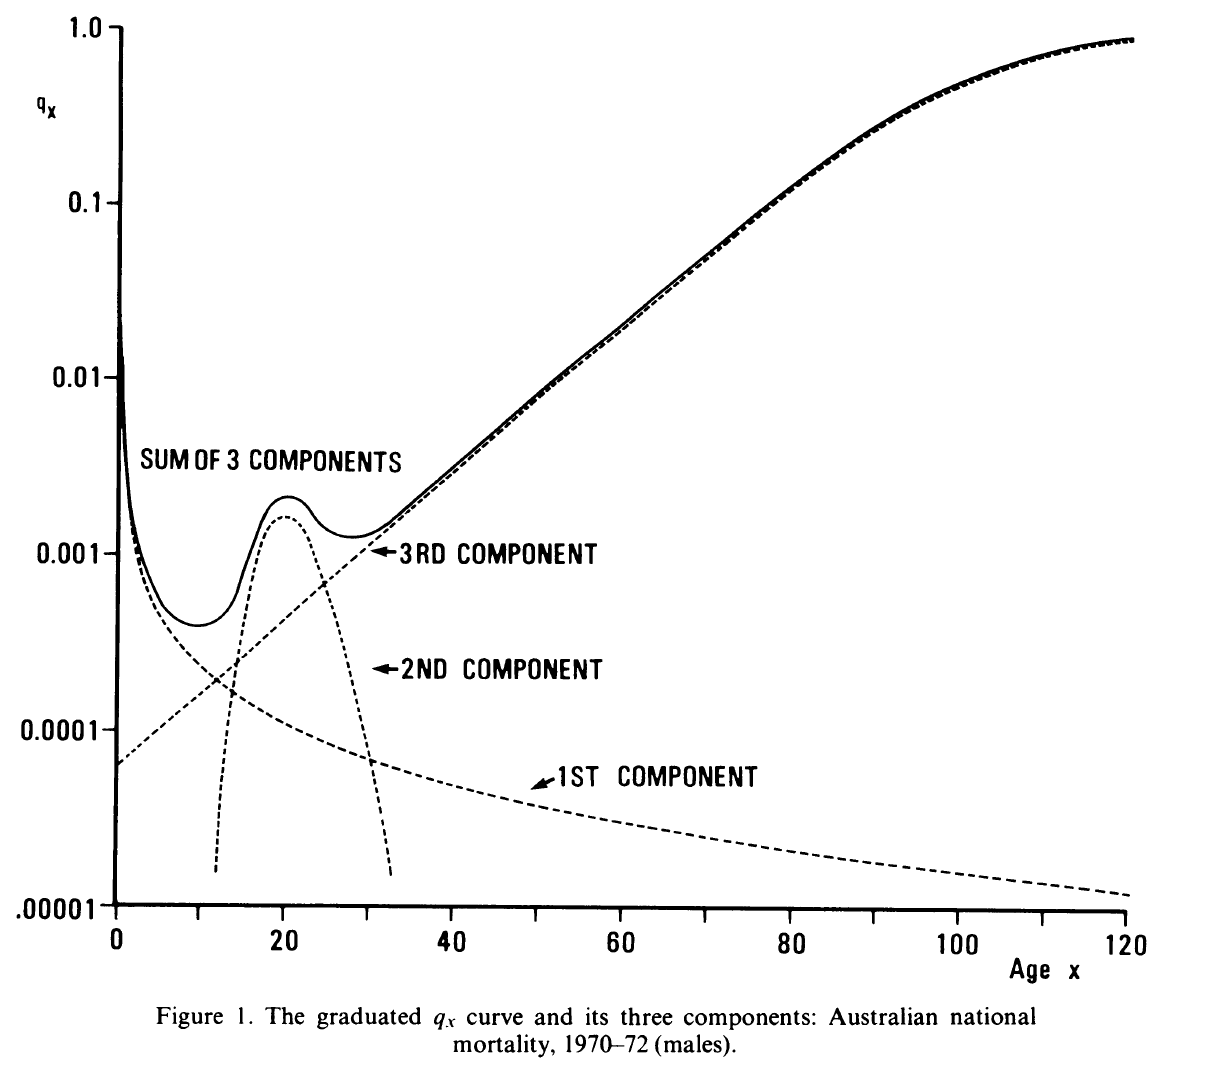
\includegraphics[width = 0.75\textwidth]{../figures/Helgman_pollard_model.png}
\caption{Illustration de l'impact de chacune des composantes du modèle de Heligman et Pollard.}
\label{fig:Helgman_pollard_model}
\end{figure}
\end{itemize}
La calibration de ces modèles se fait de deux façons
\begin{itemize}
  \item Par le maximum de vraisemblance sans utiliser les taux bruts
  \item Par les moindre carrés ordinaires, en minimisant l'écart entre les taux bruts et les taux du modèle paramétrique avec 
  $$
\argmax_{\theta\in\Theta}\sum_{x\geq 0}w_x(\widehat{q}_x - q_x(\theta))^2\text{ ou } \argmax_{\theta\in\Theta}\sum_{x\geq 0}w_x(\widehat{\mu}_x - \mu_x(\theta))^2
  $$
\end{itemize}
\begin{remark}
Pour le lissage des probabilité de décès, on peut par exemple choisir les poids inversement proportionnel de la variance des taux brut c'est à dire 
$$
w_x = \frac{E^0_x}{q_x(1-q_x)},\text{ ou }w_x = E_x^c \cdot\mu_x
$$
Cela va pénaliser les taux bruts aux grands âges.
\end{remark}
\subsection{Lissage de Whittaker-Henderson}
Il est aussi possible de lisser la série des taux bruts sans faire d'hypothèse paramétrique. On cherche à remplacer une série de donnée $y = (y_i)_{i=1,\ldots, n}$ (les probabilités de décès, les taux de décès ou une fonction de ces derniers),  par $\theta^\lambda = (\theta^\lambda_i)_{i = 1,\ldots, n}$. Le lissage de Whittaker-Henderson, expliqué par exemple dans le papier de \citet{Biessy2023}, consiste en un arbitrage entre la fidélité au données $y$ et la régularité des taux lissés $\theta^\lambda$. Les taux lissés sont solution du problème d'optimisation 
$$
\theta^\lambda = \argmax_{\theta}  F(y,w, \theta) + \lambda R(\theta),
$$
où $ w = (w_i)_{i=1,\ldots, n}$ est un vecteur de poids et $\lambda >0$ qui traduit le compromis entre fidélité $F$ et régularité $R$. Le critère de fidélité s'écrit 
$$
F(y, \theta) = \sum_{i = 1}^n w_x(y_i - \theta_i)^2.
$$
le critère de régularité est donnée par 
$$
R(\theta) = \sum_{i=0}^{n-z} (\Delta^{z}\theta)_i^2,
$$
où $(\Delta^{z}\theta)_i$ est l'operateur de différence progressive d'ordre $z$ défini par 
$$
(\Delta^{z}\theta)_i = \sum_{j=0}^z\binom{z}{j}(-1)^{z-j}\theta_{i+j}, \text{ pour }0\leq i\leq n-z. 
$$
On note que 
$$
 \Delta^{1}\theta_i = \theta_{i+1}-\theta_{i},\text{ }\Delta^{2}\theta_i =\Delta^1 \Delta^1\theta_i =\theta_i \theta_{i+2}-2\theta_{i+1}+\theta_{i},\ldots
$$
\begin{remark}
L'ordre $z$ de l'opérateur de différence progressive indique le niveau de lissage souhaité. Un polynôme de dégrée $z-1$ est ce que l'on peut obtenir de plus régulier. 
\begin{itemize}
  \item Pour $\lambda = 0$, on retrouve les taux bruts
  \item Pour $\lambda \rightarrow \infty$, on obtient le polynômes d'ordre $z-1$ qui ajuste le mieux la courbe des taux bruts suivant le critère des moindre carrés.
\end{itemize}
\end{remark}
On définit $W = \textbf{Diag}\left( w\right)$ la matrice diagonale contenant les poids. L'opérateur  de diffférence progressive $\Delta^z$ peut être représenté sous forme matricielle avec $D_{n,z}\theta = (D_{n,z}\theta)_i$ où $D_{n,z}$ est une matrice de taille $n-z\times n$. Pour $z=1$ et $z = 2$, nous avons respectivement

$$
D_{n,1} = \left(\begin{array}{cccccc}
-1&1&0&\cdots&0\\
0&-1&1&\ddots&\vdots\\
\vdots&\ddots&\ddots&\ddots&0\\
0&\cdots&0&-1&1\\
\end{array}\right).
\text{ et } D_{n,2} = \left(\begin{array}{cccccc}
-1&2&-1&0&\cdots&0\\
0&-1&2&-1&\cdots&0\\
\vdots&\ddots&\ddots&\ddots&\ddots&\vdots\\
0&\cdots&0&-1&2&-1\\
\end{array}\right).
$$
le problème d'optimisation s'écrit 
$$
\theta^\lambda = \argmin_{\theta} \mathcal{L}(\theta)= \argmin_{\theta} \,^t(y - \theta)W(y-\theta)+\lambda\,^t(D_{n,z}\theta)D_{n,z}\theta. 
$$
En notant $P_{\lambda} = \lambda \,^t D_{n,z}D_{n,z}$ (matrice carrée de taille $n^2$), on en déduit que\footnote{Voici un petit formulaire de dérivation matricielle \url{https://www.di.ens.fr/~fbach/courses/fall2009/formulaire.pdf}}
$$
\frac{\text{d} }{\text{d} \theta}\mathcal{L}(\theta) =  -2W(y - \theta)+2P_\lambda\theta
$$
Le système d'équation 
$$
\frac{\text{d} }{\text{d} \theta}\mathcal{L}(\theta)=0
$$
a pour solution
$$
\theta^\lambda = \left(W + P_\lambda\right)^{-1}Wy.
$$ 
On peut appliquer le lisage brutalement sur les probabilités de décès ou les taux brut à l'aid de la fonction \href{https://search.r-project.org/CRAN/refmans/pracma/html/whittaker.html}{whittaker} du package \texttt{pracma}. L'article de \citet{Biessy2023} rationnalise le choix  de Pour appliquer cette méthode, des observations $y$, des poids $w$, et du paramètre de lissage $\lambda$ en introduisant un modèle de statistique Bayésienne expliquer dans la \cref{app:WH}. on retiendra que 
\begin{itemize}
  \item Les données a utiliser sont
  $$
y = \log(d/E_c)\text{, et }w = d.
  $$
  \item On obtient un intervale de crédibilité suivant pour le log des taux de mortalités
  $$
\ln\mu|d,E^c\in\left[\theta^\lambda\pm\phi^{-1}\left(1-\frac{\alpha}{2}\right)\sqrt{\textbf{diag}\{(\textbf{Diag}(d)+P_\lambda)^{-1}\}}\right],
  $$
  où l'opérateur $\textbf{diag}$ extrait la diagonale et $\textbf{Diag}$ transforme un vecteur en une matrice diagonale. 
  \item Le paramètre de lissage $\lambda$ est obtenu en maximisant la vraisemblance des données.  
\end{itemize}
On peut utiliser le package \href{https://cran.r-project.org/web/packages/WH/index.html}{WH} qui comprend également une fonction permettant d'étendre la méthode en dimension $2$. C'est utile pour lisser les taux de d'entrée en incapacité ou invalidité qui prennent en compte l'ancienneté en plus de l'âge. 


\subsection{Fermeture de la table}
Le problème du manque (voir l'absence) de données aux grands âges oblige parfois d'avoir recours à des méthodes d'extrapolation. Deux méthodes sont décrites ci-après, l'idée est assez proche du lissage paramétrique. On utilise ces méthodes pour obtenir les $q_x$ aux grands âges. 

\subsubsection{Fermeture de Denuit-Goderniaux}
La méthode de \citet{Denuit2005} consiste à ajuster un modèle linéaire de la forme
$$
\log(\widehat{q}_x) = a + bx + cx^2+\epsilon_x,\text{ pour }x\in [x_{\min}, x_{\max}].
$$
où $\epsilon_x\overset{i.i.d.}{\sim}\NormalDist(0,\sigma^2)$. Les bornes $x_{\min}$ et $x_{\max}$ sont fixées de manière arbitraire par le modélisateur en fonction de la fiabilité des probabilités de décès aux grands âges. Deux conditions sont imposées
\begin{enumerate}
  \item la condition de fermeture $q_{130} = 1$
  \item la condition de concavité $q'_{130} = 0$. La probabilité de décès doit augmenter avec l'âge, cette croissance doit ralentir aux grands âges.
\end{enumerate}
Ces deux contraintes reviennent à imposer la relation suivante 
$$
a+bx+cx^2 = c(130-x)^2\text{, pour }x\in[x_{\min}, x_{\max}].
$$

\subsubsection{Fermeture de Kanisto}
La méthode de \citet{Thatcher1998} consiste à ajuster un modèle logistique de la forme
$$
\text{logit}(\widehat{q}_x) = \log\frac{q_x}{1-q_x}=\log(a) + bx,\text{ pour }x\in[x_{\min}, x_{\max}].
$$
par les moindre carrés ordinaires.
\begin{remark}
\begin{enumerate}
  \item L'ordre dans lequel on applique le lissage ou la fermeture est à la discrétion du praticien. On peut décider de lisser puis de fermer ou inversement. La fermeture peut entrainer une discontinuité dans la courbe d'où l'intérêt d'appliquer la procédure de lissage après la fermeture. L'utilisation de la fermeture sur les taux bruts peut nuire à l'estimation des paramètres d'où l'intérêt de lisser d'abord. On peut tout à fait lisser puis fermer et lisser à nouveau.
  \item La procédure de fermeture permet en premier lieu d'extrapoler les probabilités de décès aux âges non accessible. On peut également décider de remplacer les probabilités de décès des âges au dela de  $x_{\min}$ ou de  $x_{\max}$ ou encore prendre une moyenne entre taux brut et taux issus de la fermeture. Voir la note de la SOA\footnote{\url{https://www.soa.org/globalassets/assets/files/resources/essays-monographs/2005-living-to-100/m-li05-1-ix.pdf}}.
\end{enumerate}
\end{remark}
\subsection{Validation de l'ajustement}
Pour s'assurer de la qualités des taux révisés $\widehat{y}$ versus les taux bruts $y$, pouvant correspondre aux probabilités de décès ou aux taux de décès, on a recours à des tests statistiques. On effectue un test binomial (dit test des signes) pour vérifier que les taux révisés ne sont pas systématiquement au dessus ou en dessous des taux brut. On suppose que l'ajustement pour chaque âge est indépendant et on estime la probabilité $\pi$ que les taux révisé soient au dessus des taux brut par 
$$
Z = \sum_{i=1}^n\mathbb{I}_{\widehat{y}_i>y_i}.
$$
Sous 
$$
(H_0)\text{: }\pi = 1/2
$$
La statistique de test suit un loi binomial $Z\sim(n, 0.5)$. On utilise l'approximation normale 
$$
\frac{Z - np}{\sqrt{np(1-p)}}\sim\NormalDist(0,1).
$$
dès que $n$ est assez grand ($n\approx 25$). Il arive que le \textit{post-processing} des aux brut conduisent à, par exemple, une sous-estimation aux âges jeunes et une sur-estimation aux âges plus avancées. Une telle situation permet de passer le test des signes. On peut alors procéder à un autre test, appelé test des runs de Wald-Wolfowitz voir l'article wikipédia \url{https://en.wikipedia.org/wiki/Wald%E2%80%93Wolfowitz_runs_test}.

On peut comparer plusieurs méthodes de lissages en terme d'erreurs aux taux bruts en calculant par exemple des ecarts moyens quadratiques
$$
\text{MSE} = \frac{1}{n}\sum_{i = 1}^n\frac{(y_i -\widehat{y}_i)^2}{\widehat{y}_i}.
$$

\section{Evolution temporelle de la mortalité et effet cohorte}
Les tables de mortalité générationnelles sont indexés sur l'année de calendaire $t$ à laquelle les données ont été recoltées ou l'année de naissance des individus $a= t-x$.
$$
\Data =  \bigcup_{t} \{E_{x,t}, D_{x,t}\}\text{ ou } \bigcup_{a} \{E_{x,a},D_{x,a}\}
% \text{ ou } \bigcup_{t,a} \{E_{x,t, a}, D_{x,t, a}\}
$$
On peut construire autant de table de mortalité "statique" que d'année calendaire ou de cohortes disponibles. Les tables générationelles TGH et TGF $05$ comprennent des projections permettant la tarification des produits d'assurance vie. Ces tables prennent la forme de tableau à double entrée indexé sur l'âge et l'année de naissance, comme sur le \cref{tab:TGH05}.
\begin{table}[ht!]
\centering
\begin{tabular}{rrrrr}
  \hline
  Age & $1996$ & $1997$ & $1998$ &$\cdots$\\ 
  \hline
0 & 100000 & 100000 & 100000&$\cdots$ \\ 
 1 & 99607 & 99617 & 99626 &$\cdots$\\ 
 2 & 99487 & 99499 & 99510&$\cdots$ \\ 
 3 & 99435 & 99448 & 99460&$\cdots$ \\ 
 4 & 99406 & 99419 & 99432&$\cdots$ \\ 
$\vdots$ & $\vdots$ & $\vdots$ & $\vdots$&$\cdots$ \\ 
   \hline
\end{tabular}
\caption{Extrait de la table de mortalité générationnelle TGH $05$.}
\label{tab:TGH05}
\end{table}
La legislation impose l'utilisation de ces tables dans le cadre des contrats d'assurance vie comprenant des garanties du type rente viagère. 
% On peut estimer les probabilités de décès par période $t_0\in[t, t+1]$ avec 
% $$
% q_{x,t_0} = \frac{d_{x,t_0}}{E_{x,t_0}},
% $$
% par génération $a_0\in[t-x, t-x+1]$ avec
% $$
% q_{x,a_0} = \frac{d_{x,a_0}}{E_{x,a_0}},
% $$
% ou par période et par cohorte avec
% $$
% q_{x,t_0, a_0} = \frac{d_{x,t_0, a_0}}{E_{x,t_0, a_0}},
% $$
% suivant le type de données disponibles. 
La construction des tables générationnelles à partir des données bruts nécessite l'introduction d'un outil graphique: le diagramme de Lexis, voir \cref{fig:lexis_1}.
\subsection{Diagramme de Lexis}
Le parcours des individus d'une population est représenté sur un diagramme de Lexis 
\begin{itemize}
\item Abscisse: $t = $ année calendaire ,
\item Ordonnée: $x=$ âge,
\end{itemize}

% \begin{figure}[!ht]
% \begin{center}
% \begin{tikzpicture}
% \draw[->] (-1,0) -- (5,0);
% \draw (5,0) node[right] {t};
% \draw [->] (0,-1) -- (0,5);
% \draw (0,5) node[above] {$x$};
% \draw [dashed] (4,3) -- (0,3)  node[left] {$x_0$};
% \draw [dashed] (4,3) -- (4,0) node[below] {$t_0$};
% \draw [solid] (4,3) node{ \color{black}$\bullet$} -- (1,0) node[below] {$t_0-x_0$};
% \end{tikzpicture}
% \caption{Positionnement d'un individu qui décède à l'age $x_0$ durant l'année $t_0$ sur le diagramme de Lexis}
% \label{fig:lexis_1}
% \end{center}
% \end{figure}
% Lorsque les données sont exhaustives on peut représenter précisément le parcours de chaque individu sur le diagramme. 
% \begin{figure}
% \begin{center}
% \begin{tikzpicture}
% \draw[->] (0,0) -- (6.5,0);
% \draw [->] (0,0) -- (0,6.5);
% % Grid
% \draw [color=gray!80] (1,0) node[below] {$t-1$} -- (1,6.5);
% \draw [color=gray!80] (3,0) node[below] {$t$} -- (3,6.5);
% \draw [color=gray!80] (5,0) node[below] {$t+1$} -- (5,6.5);
% \draw [color=gray!80] (0,1) node[left] {$x-1$} -- (6.5,1);
% \draw [color=gray!80] (0,3) node[left] {$x$} -- (6.5,3);
% \draw [color=gray!80] (0,5) node[left] {$x+1$} -- (6.5,5);
% % 
% \draw plot[domain=0:4] (\x, 3+\x);
% \draw plot[domain=0:5.2] (\x, 1.8+\x);
% \draw plot[domain=0:3.4] (\x, 1.2+\x) node[] {$\bullet$};
% \draw plot[domain=0.5:4.7] (\x, -0.5+\x) node[] {$o$};
% \draw plot[domain=1.2:6.5] (\x, -1.2+\x) node[] {};
% \draw plot[domain=1.4:5.2] (\x, -1.4+\x) node[] {$\bullet$};
% \draw plot[domain=3:6] (\x, -3+\x) node[] {$\bullet$};
% \draw plot[domain=4.25:6.5] (\x, -4.25+\x) node[] {};
% \draw plot[domain=0:2] (\x, 3+\x) ;
% \end{tikzpicture}
% \caption{Parcours des individus sur le diagramme de Lexis. $\bullet=$  décès et $o=$ fin d'observation de l'individu (censure à droite)}
% \label{fig:lexis}
% \end{center}
% \end{figure}
% l'estimation des taux de mortalité se résume à compter le nombre de décès ($\bullet$) dans les triangles, les carrés ou les parallélogrammes du diagramme de Lexis suivant que l'on calcule des taux de décès pour
% \begin{itemize}
%   \item une période $t_0\in[t, t+1)$: carré de Lexis
%   \item cohorte $a_0\in[t-x, t-x+1)$: parallélogramme de Lexis
%   \item période et cohorte $(t_0,a_0)\in[t, t+1)\times [t-x, t-x+1)$: triangle de Lexis
% \end{itemize}
% puis à rapporter ce nombre sur l'exposition au risque. Lorsque l'on connait la date exacte des décès, l'exposition est le cumul des longueurs des segments des parcours passant au travers du carré, triangle ou parallélogramme étudié, voir la \cref{fig:lexis_geom}. 
% \begin{figure}[ht!]
% \begin{center}
% \begin{tikzpicture}
% \draw[->] (0,0) -- (6.5,0);
% \draw [->] (0,0) -- (0,6.5);
% % Grid
% \draw [color=gray!80] (1,0) node[below] {$t-1$} -- (1,6.5);
% \draw [color=gray!80] (3,0) node[below] {$t$} -- (3,6.5);
% \draw [color=gray!80] (5,0) node[below] {$t+1$} -- (5,6.5);
% \draw [color=gray!80] (0,1) node[left] {$x-1$} -- (6.5,1);
% \draw [color=gray!80] (0,3) node[left] {$x$} -- (6.5,3);
% \draw [color=gray!80] (0,5) node[left] {$x+1$} -- (6.5,5);
% % 

% \draw[-, dashed] plot[domain=0:5] (\x, 1.2+\x)  node[above left] {};
% \draw[->] plot[domain=0:2.5] (\x, 1.2+\x)  node[above left] {$t-x-1$};
% \draw[-,, dashed] plot[domain=0.5:6] (\x, -0.5+\x) node[below right] {};
% \draw[->] plot[domain=0.5:2.5] (\x, -0.5+\x) node[below right] {$t-x$};
% \draw [-, very thick] (3,3) -- (5,5);
% \draw [very thick] (3,3) -- (3,5) -- (5,5) -- (5,3) -- cycle;
% \draw [very thick] (5,3) -- (5,5) -- (7,5) -- cycle;
% \end{tikzpicture}
% \caption{Géométrie de Lexis}
% \label{fig:lexis_geom}
% \end{center}
% \end{figure}
% Les individus de la cohorte nés l'année $t-x$ atteindrons l'âge $x$ durant les années calendaires $t$ et $t+1$.

\subsection{Taux de mortalité par période}
Considérons les évènements se produisant sur la période $[t, t+1]$, nous intéressons au carré de Lexis de la \cref{fig:lexis_square}
\begin{figure}
\begin{center}
\begin{tikzpicture}
\draw[->] (0,0) -- (6.5,0);
\draw [->] (0,0) -- (0,6.5);
% Grid
\draw [color=gray!80] (1,0) node[below] {$t-1$} -- (1,6.5);
\draw [color=gray!80] (3,0) node[below] {$t$} -- (3,6.5);
\draw [color=gray!80] (5,0) node[below] {$t+1$} -- (5,6.5);
\draw [color=gray!80] (0,1) node[left] {$x-1$} -- (6.5,1);
\draw [color=gray!80] (0,3) node[left] {$x$} -- (6.5,3);
\draw [color=gray!80] (0,5) node[left] {$x+1$} -- (6.5,5);
% 
\draw plot[domain=0:4] (\x, 3+\x);
\draw plot[domain=0:5.2] (\x, 1.8+\x);
\draw plot[domain=0:3.4] (\x, 1.2+\x) node[] {$\bullet$};
\draw plot[domain=0.5:4.7] (\x, -0.5+\x) node[] {$o$};
\draw plot[domain=1.2:6.5] (\x, -1.2+\x) node[] {};
\draw plot[domain=1.4:5.2] (\x, -1.4+\x) node[] {$\bullet$};
\draw plot[domain=3:6] (\x, -3+\x) node[] {$\bullet$};
\draw plot[domain=4.25:6.5] (\x, -4.25+\x) node[] {};
\draw plot[domain=0:2] (\x, 3+\x) ;
\draw [blue, very thick] (3,3)    -- (3,5) ;
\draw [red, very thick] (3,3) -- (5,3) node[above left] {\color{red}$ D^L_{x,t}$};
\draw [red, very thick] (5,5) -- (5,3)  ;
\draw [blue, very thick] (3,5) node[below right] {\color{blue}$D^U_{x,t}$}  -- (5,5)   ;
 % --  -- cycle;
\end{tikzpicture}
\caption{Parcours des individus sur le diagramme de Lexis. $\bullet=$  décès et $o=$ fin d'observation de l'individu (censure à droite)}
\label{fig:lexis_square}
\end{center}
\end{figure}
\begin{itemize}
% \item $P_{x,t} = 2$ est le nombre d'individu d'âge $x$ au début de la période $t$. Il s'agit du nombre de segments intersectant le côté $(x,t) - (t,x+1)$.
\item $D^U_{x,t}=1$ compte le nombre de décès d'individu d'âge $x$ au début de la période $[t, t+1]$
\item $D^L_{x,t}=0$ compte le nombre de décès d'individu d'âge $x-1$ atteignant l'âge $x$ durant la période $[t, t+1]$.
\item Le nombre de décès au cours de la période est donné par 
$$
D_{x,t} = D^U_{x,t} + D^L_{x,t} = 1.
$$
\end{itemize} 
L'exposition exacte est donnée par la somme des longueurs des segments (divisé par $\sqrt{2}$) dans le carré de Lexis, ici 
$$
E_{x,t} =  0.08 + 0.3 + 0.6 + 0.42 + 0.33 = 1.73.
$$
La probabilité de décès d'un individu d'âge $x$ durant la période $[t, t+1]$ est égale à 
$$
\mu_{x,t} = \frac{1}{1.73} = 0.57.
$$
\begin{remark}
L'estimateur prenant en compte la longueur de segment pour le calcul de l'exposition est l'estimateur de \citet{Hoem1971}. Il est très utilisé en sciences actuarielle, une comparaison avec l'estimateur de Kaplan-Meier dans le cadre d'une application à la mortalité est proposé dans \citet{Guibert2017}. La méthodologie ci-après suit le protocole de calcul établi dans le cadre du projet HMD\footnote{\url{https://www.mortality.org/}} voir \citet{Wilmoth2007}. 
\end{remark}
Si les longueurs de segments ne sont pas accessible l'exposition est approchée en sommant l'exposition des trianges supérieurs et inférieur avec 
$$
E_{x,t} = E_{x,t}^L + E_{x,t}^U.
$$
L'exposition du triangle inférieur comprend $P_{x,t+1}$ la population d'âge $x$ au début de l'année $t+1$ auquel nous devons ajouter la contribution des décès du triangle inférieur. On a 
$$
E_{x,t}^L = l_1P_{x,t+1}+l_2D^{L}_{x,t}.
$$
L'exposition du triangle supérieur comprend $P_{x,t}$ la population d'âge $x$ au début de l'année $t$ à laquelle nous devons soustraire la contribution des décès du triangle supérieur.  
$$
E_{x,t}^U = u_1P_{x,t}-u_2D^{U}_{x,t}.
$$
Les coefficients l$_1, l_2, u_1$ et $u_2$ peuvent être inférés à l'aide de la distribution des naissance pour les cohortes $t-x-1$ et $t-x$ comme sur la \cref{fig:Lexis_expo_computation}. 
\begin{figure}[h!] 
\centering
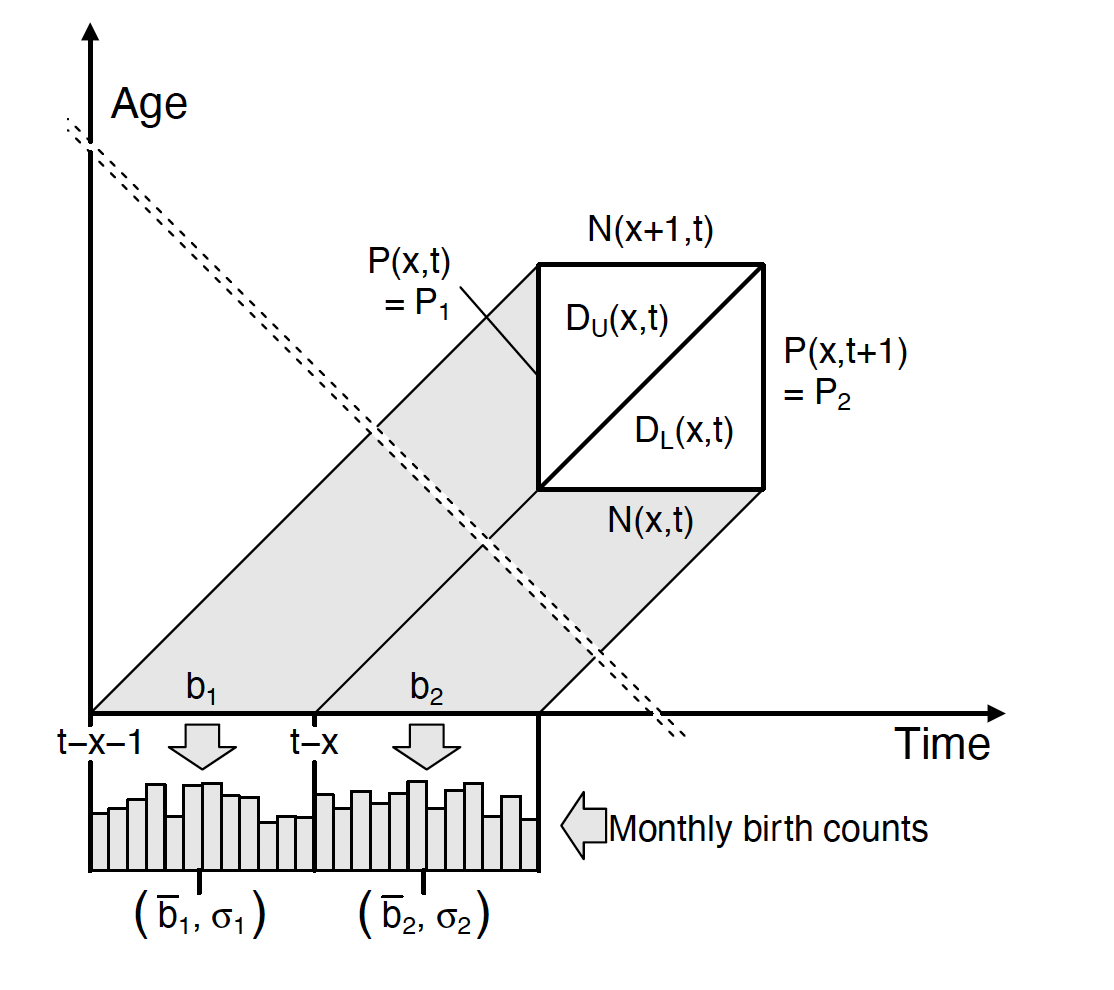
\includegraphics[width = 0.75\textwidth]{../figures/Lexis_expo_computation.png}
\caption{Calcul d'exposition central sur un diagrame de Lexis grâce à la distribution des naissances pour les cohortes concernées. (Source: HMD Documentation)}
\label{fig:Lexis_expo_computation}
\end{figure}
Soit $B_1,B_2\in[0,1]$ les \va qui indiquent la répartition des naissances au sein de la cohorte $t-x-1$ et $t-x$ respectivement. Soient $f_{B_1}$ et $f_{B_2}$ les densités de $B_1$ et $B_2$. On note également 
$$
\bar{b}_i = \E(B_i),\text{ et }\sigma_i^2 = \V(B_i),\text{ pour }i = 1,2.
$$
Dans le triangle inférieur, la contribution à l'exposition des individus d'âge $x$ au temps $t+1$ est donnée par 
\begin{equation}\label{eq:expos_contribution_lower}
\E\left[1-B_2\right] = (1-\bar{b}_2), 
\end{equation}
La contribution des décès est un peu plus subtil. Un décès dans le triangle inférieur est un point $(t+U, x+V)$ avec $(U,V)$ un couple de variable aléatoire telle que $0\leq V\leq U\leq 1$. On suppose que la densité jointe de $(U,V)$ est donnée par 
\begin{equation}\label{eq:joint_density_lower}
f_{(U,V)}(u,v) = C_L f_{B_{2}}(u-v)\mathbb{I}_{0\leq v\leq u\leq 1}(u,v),
\end{equation}
où $C_L$ est une constante de normalisation. Ce choix entraine que 
\begin{itemize}
  \item La probabilité que le décès survienne est constante le long de la ligne de vie
  \item La densité est proportionelle à la densité de probabilité de $B_2$
\end{itemize}
En intégrant \eqref{eq:joint_density_lower}, on identifie $C_L = 1/(1-\bar{b}_{2})$. Pour un décès qui a lieu au point $(t+U, x+V)$, la perte d'exposition est donnée par 
\begin{equation}\label{eq:lost_exposure_death_lower}
\int_{0}^1\int_{0}^u(1-u)\frac{f_{B_2}(u-v)}{1 - \bar{b_2}}\text{d}v\text{d}u = \frac{1-\bar{b}_2}{2}+\frac{\sigma_2^2}{2(1-\bar{b}_2)}
\end{equation}
On déduit de \eqref{eq:expos_contribution_lower} et \eqref{eq:lost_exposure_death_lower} l'exposition dans le triangle inférieur avec 
\begin{eqnarray*}
E^L_{x,t}&=&(1-\bar{b}_2)(P_{x,t+1}+D^L_{x,t}) - \left(\frac{1-\bar{b}_2}{2}+\frac{\sigma_2^2}{2(1-\bar{b}_2)}\right)D^L_{x,t}\\
& =& (1-\bar{b}_2)P_{x,t+1} + \left(\frac{1-\bar{b}_2}{2}-\frac{\sigma_2^2}{2(1-\bar{b}_2)}\right)D^L_{x,t}\\
&=& l_1P_{x,t+1} + l_2 D^L_{x,t}
\end{eqnarray*}

Dans le triangle supérieur, la contribution des individus d'âge $x$ à l'année $t$ à l'exposition  est donnée par 
\begin{equation}\label{eq:expos_contribution_upper}
\E\left(B_1\right)=\bar{b}_1.
\end{equation}
Un décès dans le triangle supérieur est un point $(t+U, x+ V)$ avec $0\leq U\leq V\leq 1$. La densité jointe de $(U,V)$ est donnée par (pour les mêmes raison que précédemment)
\begin{equation}\label{eq:joint_density_upper}
f_{(U,V)}(u,v) = C_U f_{B_{1}}(u+1-v)\mathbb{I}_{0\leq u\leq v\leq 1}(u,v),
\end{equation}
En intégrant \eqref{eq:joint_density_upper}, on identifie $C_U = 1/\bar{b}_{1}$. Pour un décès qui a lieu au point $(t+U, x+V)$, le gain d'exposition est donnée par 
\begin{equation}\label{eq:lost_exposure_death_upper}
\int_{0}^1\int_{u}^1u\frac{f_{B_1}(u+1-v)}{\bar{b}_1}\text{d}v\text{d}u = \frac{\bar{b}_1}{2}+\frac{\sigma_1^2}{2\bar{b}_1}
\end{equation}
On déduit de \eqref{eq:expos_contribution_upper} et \eqref{eq:lost_exposure_death_upper} l'exposition dans le triangle inférieur avec 
\begin{eqnarray*}
E^U_{x,t}&=&\bar{b}_1(P_{x,t}-D^U_{x,t}) + \left(\frac{\bar{b}_1}{2}+\frac{\sigma_1^2}{2\bar{b}_1}\right)D^U_{x,t}\\
& =& \bar{b}_1P_{x,t} - \left(\frac{\bar{b}_1}{2}-\frac{\sigma_1^2}{2\bar{b}_2}\right)D^U_{x,t}\\
&=& u_1P_{x,t} - u_2 D^U_{x,t}
\end{eqnarray*}

En l'absence d'information sur la distribution des naissances au cours des l'années au sein des cohortes, on suppose que $B_1,B_2\sim\UnifDist(0,1)$. Il vient alors
$$
E_{x,t} \approx  \frac{1}{2}[P_{x,t}+ P_{x,t+1}] + \frac{1}{6}[D^L_{x,t}- D^U_{x,t}] = 1.7.
$$
La probabilité de décès d'un individu d'âge $x$ durant la période $[t, t+1]$ est égale à 
$$
\widehat{\mu}_{x,t} = \frac{1}{1.7} = 0.59.
$$
\begin{remark}
Si nous n'avons accès qu'au nombre de décès $D_{x,t}$ d'individus d'âge $x$ pendant l'année $t$ alors on peut considérer que $D^U_{x,t} = D^L_{x,t} = D_{x,t} / 2$. Pour plus de détail sur les calculs d'exposition en prenant en compte les données de natalité, voir le travail de \citet{Boumezoued2020}.
\end{remark}
\subsection{Taux de mortalité par cohorte}
Considérons les évènements concernant les individus d'âge $x$ nés l'année $a=t-x$, nous intéressons au parallélogramme de Lexis de la \cref{fig:lexis_para}
\begin{figure}
\begin{center}
\begin{tikzpicture}
\draw[->] (0,0) -- (6.5,0);
\draw [->] (0,0) -- (0,6.5);
% Grid
\draw [color=gray!80] (1,0) node[below] {$t-1$} -- (1,6.5);
\draw [color=gray!80] (3,0) node[below] {$t$} -- (3,6.5);
\draw [color=gray!80] (5,0) node[below] {$t+1$} -- (5,6.5);
\draw [color=gray!80] (0,1) node[left] {$x-1$} -- (6.5,1);
\draw [color=gray!80] (0,3) node[left] {$x$} -- (6.5,3);
\draw [color=gray!80] (0,5) node[left] {$x+1$} -- (6.5,5);
% 
\draw plot[domain=0:4] (\x, 3+\x);
\draw plot[domain=0:5.2] (\x, 1.8+\x);
\draw plot[domain=0:3.4] (\x, 1.2+\x) node[] {$\bullet$};
\draw plot[domain=0.5:4.7] (\x, -0.5+\x) node[] {$o$};
\draw plot[domain=1.2:6.5] (\x, -1.2+\x) node[] {};
\draw plot[domain=1.4:5.2] (\x, -1.4+\x) node[] {$\bullet$};
\draw plot[domain=3:6] (\x, -3+\x) node[] {$\bullet$};
\draw plot[domain=4.25:6.5] (\x, -4.25+\x) node[] {};
\draw plot[domain=0:2] (\x, 3+\x) ;
\draw [blue, very thick] (5,5) node[above right] {\color{blue}$D^U_{x,t+1}$} -- (7,5);
\draw [blue, very thick] (5,3)-- (7,5);
\draw [red, very thick] (3,3) -- (5,3) node[above left] {\color{red}$ D^L_{x,t}$};
\draw [red, very thick] (3,3) -- (5,5) ;
\draw [black, very thick] (5,5) -- (5,3) ;
% \draw [blue, very thick] (3,5)   -- (5,5)  ;
 % --  -- cycle;
\end{tikzpicture}
\caption{Parcours des individus sur le diagramme de Lexis. $\bullet=$  décès et $o=$ fin d'observation de l'individu (censure à droite)}
\label{fig:lexis_para}
\end{center}
\end{figure}
L'exposition est donnée par la somme des longueurs des segments dans le parallélogramme, soit 
$$
E_{x,a} = 0.8+1+0.4 =2.2.
$$
La probabilité de décès des individus d'âge $x$ né l'année $a$ est donnée par 
$$
q_{x,a} = 1/2.2 = 0.45.
$$

Si la longueur des segments est inconnue alors au vu des calculs effectués pour les taux de mortalité par période, il vient
$$
E_{x,a}= P_{x,t+1} + \left(\frac{1-\bar{b}}{2}+\frac{\sigma^2}{2(1-\bar{b})}\right)D^L_{x,t} -  \left(\frac{\bar{b}}{2}+\frac{\sigma^2}{2\bar{b}}\right)D^U_{x,t+1}
$$
avec $a =t-x$, voir \cref{fig:death_rate_cohort_HMD}.
\begin{figure}[h!] 
\centering
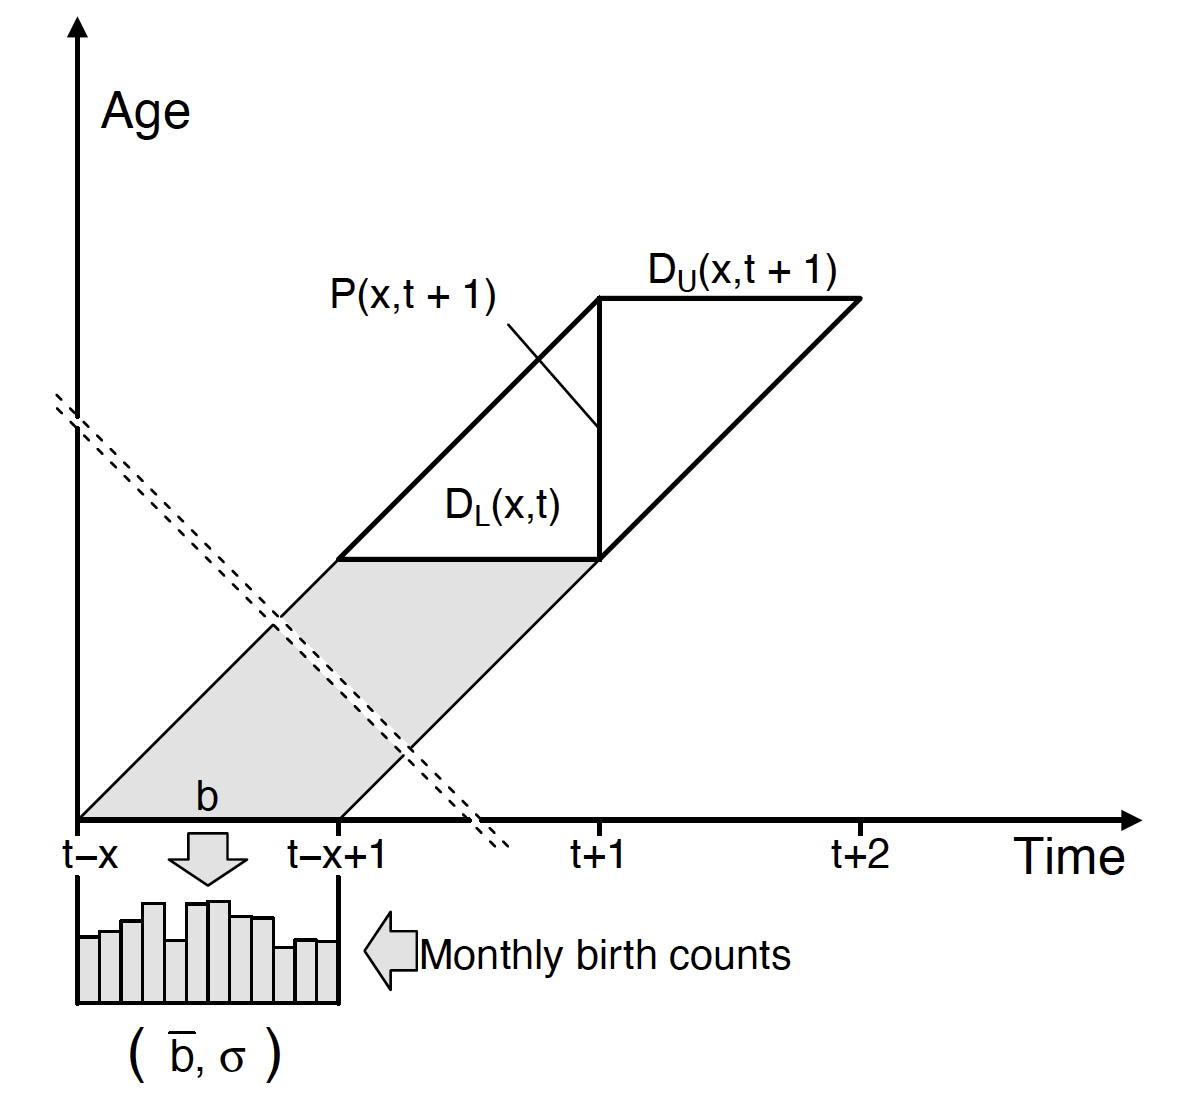
\includegraphics[width = 0.75\textwidth]{../figures/death_rate_cohort_HMD.png}
\caption{Calcul d'exposition central sur un diagrame de Lexis grâce à la distribution des naissances pour la cohortes concernée. (Source: HMD Documentation)}
\label{fig:death_rate_cohort_HMD}
\end{figure}
Si l'information sur les moments de la distribution des naissances n'est pas disponible alors on suppose une distribution uniforme qui mène à la simplification suivante 
$$
E_{x,a}= P_{x,t+1} + \frac{1}{3}(D^L_{x,t} - D^U_{x,t+1})
$$
puis
$$
\widehat{q}_{x,a} = 1/2 = 0.5.
$$ 
% \subsection{Taux de décès par période et cohorte}
% Considérons les évènements concernant les individus d'âge $x$,  nés l'année $a=t-x$, durant la période $[t,t+1]$. Nous nous intéressons au triangle de Lexis de la \cref{fig:lexis_triangle}
% \begin{figure}
% \begin{center}
% \begin{tikzpicture}
% \draw[->] (0,0) -- (6.5,0);
% \draw [->] (0,0) -- (0,6.5);
% % Grid
% \draw [color=gray!80] (1,0) node[below] {$t-1$} -- (1,6.5);
% \draw [color=gray!80] (3,0) node[below] {$t$} -- (3,6.5);
% \draw [color=gray!80] (5,0) node[below] {$t+1$} -- (5,6.5);
% \draw [color=gray!80] (0,1) node[left] {$x-1$} -- (6.5,1);
% \draw [color=gray!80] (0,3) node[left] {$x$} -- (6.5,3);
% \draw [color=gray!80] (0,5) node[left] {$x+1$} -- (6.5,5);
% % 
% \draw plot[domain=0:4] (\x, 3+\x);
% \draw plot[domain=0:5.2] (\x, 1.8+\x);
% \draw plot[domain=0:3.4] (\x, 1.2+\x) node[] {$\bullet$};
% \draw plot[domain=0.5:4.7] (\x, -0.5+\x) node[] {$o$};
% \draw plot[domain=1.2:6.5] (\x, -1.2+\x) node[] {};
% \draw plot[domain=1.4:5.2] (\x, -1.4+\x) node[] {$\bullet$};
% \draw plot[domain=3:6] (\x, -3+\x) node[] {$\bullet$};
% \draw plot[domain=4.25:6.5] (\x, -4.25+\x) node[] {};
% \draw plot[domain=0:2] (\x, 3+\x) ;
% % \draw [blue, very thick] (5,5) node[below right] {\color{blue}$D^U_{x,t}$} -- (7,5);
% % \draw [blue, very thick] (5,3)-- (7,5);
% \draw [red, very thick] (3,3) -- (5,3) node[above left] {\color{red}$ D^L_{x,t}$};
% \draw [red, very thick] (3,3) -- (5,5) ;
% \draw [red, very thick] (5,5) -- (5,3) ;
% % \draw [blue, very thick] (3,5)   -- (5,5)  ;
%  % --  -- cycle;
% \end{tikzpicture}
% \caption{Parcours des individus sur le diagramme de Lexis. $\bullet=$  décès et $o=$ fin d'observation de l'individu (censure à droite)}
% \label{fig:lexis_triangle}
% \end{center}
% \end{figure}
% L'exposition est donnée par la somme des longueurs des segments dans le triangle, soit 
% $$
% L^c(x,a) \approx 0.8 + 0.4 + 0.3 = 1.5
% $$
% La probabilité de décès des individus d'âge $x$ né l'année $a$ est donnée par 
% $$
% q_{x,a} = 0/1.5 = 0.
% $$
% Si la longueur des segments est inconnue alors on fait l'approximation suivante 
% $$
% L^c(x,a) \approx L_{x,t+1} - \frac{1}{2}D^L_{x,t}  = 2
% $$
% et
% $$
% \widehat{q}_{x,a} = 0/2 = 0.
% $$ 
\subsection{Modèle de projection de la mortalité}
L'objectif est de rendre compte de la tendance des taux de mortalité $\mu_{x,t}$ et probabilités de décès $q_{x,t}$ au cours du temps. Dans la section précédente, nous avons estimé des expositions dites centrales $E_{x,t}^c$. Les taux de mortalités sont estimés sur la base de l'exposition centrale avec 
$$
\mu_{x,t} = \frac{D_{x,t}}{E_{x,t}^c}.
$$
Les probabilité de décès requiert usuellement l'exposition initiale $E_{x,t}^0$ avec 

$$
q_{x,t} = \frac{D_{x,t}}{E_{x,t}^0}.
$$
Les deux expositions sont approximativement lié par $E_{x,t}^0\approx E_{x,t}^c +D_{x,t}/2$. On utilisera la notation $E_{x,t}$ pour l'exposition centrale ou initiale lorsque le contexte est clair. Les probabilité de décès et taux de mortalité sont liés par
$$
q_{x,t}=1-\exp(-\mu_{x,t}).
$$
Les modèles de mortalité stochastiques, aussi appelé GAPC (\textit{Generalized} Age-Period-Cohort comprennent $4$ composantes.
\begin{enumerate}  
  \item Une composante aléatoire  
  $$
D_{x,t}\sim \PoissonDist(\mu_{x,t}\cdot E_{x,t}^c)\text{, avec }\E(D_{x,t}) = E_{x,t}^c\cdot \mu_{x,t},
  $$
  ou
  $$
D_{x,t}\sim \BinomialDist( E_{x,t}^0, q_{x,t})\text{, avec }\E(D_{x,t}) = E_{x,t}^0\cdot q_{x,t},
  $$
  \item Une composante systématique
  $$
\eta_{x,t} = \alpha_x + \sum_{i=1}^N \beta_{x}^{(i)}\kappa_{t}^{(i)}+\beta_{x}^{(0)}\gamma_{t-x},
  $$
  où
  \begin{itemize}
    \item Le terme $\alpha_x$ caractérise l'effet statique de l'âge sur la mortalité
    \item $N$ est le nombre de terme de type age-période. Les termes $\kappa_t^{(i)},\text{ }i=1,\ldots, N$ décrivent la tendance de la mortalité au cours du temps modulé par l'âge via les termes $\beta_x^{(i)}$
    \item Le terme $\gamma_{t-x}$ tient compte d'un possible effet cohorte modulé par l'âge via le terme $\beta_{x}^{(0)}$.
  \end{itemize}
  Les termes age-dépendant $\beta_x^{i}$ peuvent être des fonctions prédeterminé de l'âge $\beta_x^{i} = f^{i}(x)$ ou bien des coefficients sans structures préalables. Les termes périodes-dépendant $\kappa_t^{i}$ et cohortes-dépendants $\gamma_{t-x}$ sont considérés comme des processus stochastiques. Les méthodes d'études des série chronologiques s'appliquent pour effectuer les prévisions de l'évolution de la mortalité. Cette structure permet de prendre en compte la plupart des modèles de mortalités, voir \citet{Hunt2020}.
  \item La fonction de lien $g$ entre la composante aléatoire et la composante systématique avec 
  $$
  g\left[\E\left(\frac{D_{x,t}}{E_{x,t}}\right)\right] =  \eta_{x,t}.
  $$
  Dans le cadre du modèle de Poisson, on utilise la fonction log\footnote{$\log(\mu_{x,t})$}. Pour le modèle binomial la fonction logit\footnote{$\log(q_{x,t}/(1-q_{x,t}))$}. Ce sont les fonctions de lien canonique des modèles linéaires généralisés, voir \citet{Currie2014} pour une discussion sur les fonctions de liens dans le cadre des modèles de mortalités stochastiques.
  \item Les contraintes sur les paramètres permettant de rendre le modèle identifiable. On applique au vecteur de paramètres
  $$
  \theta = \left(\alpha_x,\beta_{x}^{(1)},\ldots, \beta_x^{(N)},\kappa_{t}^{(1)},\ldots, \kappa_{t}^{(N)}, \beta^{(0)}, \gamma_{t-x}\right)
  $$
  une transformation $v$ avec 
$$
  \tilde{\theta} = \left(\tilde{\alpha}_x,\tilde{\beta}_{x}^{(1)},\ldots, \tilde{\beta}_x^{(N)},\tilde{\kappa}_{t}^{(1)},\ldots, \tilde{\kappa}_{t}^{(N)}, \tilde{\beta}^{(0)}, \tilde{\gamma}_{t-x}\right).
$$
La conséquence est une perte de degré de liberté sans changer le prédicteur $\eta_{x,t}$.
\end{enumerate}

\begin{ex}
Voici quelques exemples de modèles de type GAPC.
\begin{enumerate}
  \item Dans le modèle de \citet{Lee1992}, on utilise le modèle de Poisson et le prédicteur est donnée par 
  $$
  \eta_{x,t} = \alpha_x +\beta_x\kappa_t.
  $$
  La composante temporelle est modélisée par une marche aléatoire avec une tendance, c'est à dire 
  $$
  \kappa_t = \delta + \kappa_{t-1}+ \epsilon_t,\text{ avec }\epsilon_t\sim\NormalDist(0,\sigma^2).
  $$
  Le modèle de Lee-Carter n'est pas identifiable au sens où la transformation 
  $$
  (\alpha_x\text{, }\beta_x\text{, }\kappa_t)\mapsto\left(\alpha_x + c_1\beta_x\text{, } \frac{\beta_x}{c_2}\text{, } c_2(\kappa_t-c_1)\right)
  $$
  n'a aucun effet sur les $\eta_{x,t}$. On impose donc les conditions suivante 
  $$
  \sum_x \beta_x=1 \text{ et }\sum_t\kappa_t =0,
   $$
   ce qui revient à fixer $c_1$ et $c_2$ de la façon suivante
   $$
   c_1=\frac{1}{n}\sum_{t}\kappa_t\text{, et }c_2 = \sum_x\beta_x,
   $$
   où $n$ est le nombre d'année d'historique.
  \item Le modèle APC, voir \citet{Clayton1987}, s'appuie aussi sur le modèle de Poisson et suppose que 
  $$
  \eta_{x,t}= \alpha_x + \kappa_t + \gamma_{t-x}.
  $$
  Le modèle APC n'est pas identifiable car il est invariant par rapport aux deux transformations suivantes
  $$
  (\alpha_x\text{, }\text{, }\kappa_t\text{, }\gamma_{t-x})\mapsto\left(\alpha_x + \phi_1-\phi_2x\text{, } \kappa_t+\phi_2 t\text{, } \gamma_{t-x}-\phi_1 - \phi_2(t-x)\right)
  $$
  et 
  $$
  (\alpha_x\text{, }\kappa_t\text{, }\gamma_{t-x})\mapsto\left(\alpha_x + c_1\text{, } \kappa_t-c_1\text{, } \gamma_{t-x}\right),
  $$
  où $c_1,\phi_1$ et $\phi_2$ sont des constantes dans $\RL$. L'identifiabilité est obtenue en imposant les contraintes suivantes
  $$
\sum_{t}\kappa_t = 0\text{, }\sum_{a=t_1-x_k}^{t_n-x_1}\gamma_a=0\text{, }\sum_{a=t_1-x_k}^{t_n-x_1}a\gamma_a=0,
$$
où $x_1 = \min x$, $t_1=\min t$, $x_k = \max x$ et $t_n = \max t_n$. L'effet cohorte fluctue autour de $0$ sans faire apparaître de tendance. Les contraintes sont imposées d'abord par une regression linéaire de $\gamma_{t-x}$ sur $t-x$ avec 
$$
\gamma_{t-x} = \phi_1 + \phi_2(t-x) + \epsilon_{t-x},\text{ }\epsilon_{t-x}\sim\NormalDist(0,\sigma^2).
$$
puis la contrainte sur la composante temporelle
$$
c_1 = \frac{1}{n}\sum_t\kappa_t,
$$
\item Le modèle CBD de \citet{Cairns2006} s'appuie sur le modèle binomiale et un prédicteur donné par 
$$
\eta_{x,t} = \kappa_t^{(1)} + (x-\bar{x})\kappa_t^{(2)}.
$$
Les composantes temporelles sont modélisés par une marche aléatoire bivariée. Ce modèle est identifiable donc aucune contrainte n'est imposée.
\end{enumerate}
\end{ex}
Les modèles sont ajustées au données via le maximum de vraisemblance via le package StMoMo, voir \citet{Villegas2018}. Soit $\Data = (D_{x,t}, E_{x,t})_{x,t}$ les données disponibles et $\theta = (\mu_{x,t})_{x,t}\text{ ou }(q_{x,t})_{x,t}$ les paramètres. La vraisemblance s'écrit 
$$
\mathcal{L}(\Data;\theta) = \sum_x\sum_t w_{x,t}\left\{D_{x,t}\log(\mu_{x,t}E_{x,t})-E_{x,t}\mu_{x,t}-\log(D_{x,t}!)\right\}
$$
dans le modèle de Poisson et 
$$
\mathcal{L}(\Data;\theta) = \sum_x\sum_t w_{x,t}\left\{\log\binom{E_{x,t}}{D_{x,t}} + D_{x,t}\log(q_{x,t}) + (E_{x,t} - D_{x,t})\log(1-q_{x,t})\right\}.
$$
dans le modèle binomial, avec 
$$
w_{x,t} = \begin{cases}
1,& \text{ si l'observation } (x,t)\text{ est utilisée pour la calibration},\\
0,& \text{ sinon.}
\end{cases}
$$
L'ajustement du modèle est mesuré à l'aide des résidus définis, pour chaque observation $(x,t)$ par 
$$
r_{x,t} = \text{sign}(D_{x,t} - \widehat{D}_{x,t})\sqrt{\frac{\text{dev}(x,t)}{\phi}},
$$
où 
\begin{itemize}
  \item $\widehat{D}_{x,t} = \widehat{\mu}_{x,t}E_{x,t}^c\text{ ou }\widehat{q}_{x,t}E_{x,t}^0$ est la prédiction du modèle
  \item La déviance en chaque point $(x,t)$ est donnée par
  $$
      \text{dev}(x,t)=\begin{cases}
      2\left[D_{x,t}\log\left(\frac{D_{x,t}}{\widehat{D}_{x,t}}\right)- (D_{x,t} - \widehat{D}_{x,t})\right]&\text{ pour le modèle de Poisson},\\
      2\left[D_{x,t}\log\left(\frac{D_{x,t}}{\widehat{D}_{x,t}}\right)+(E_{x,t}^0 - D_{x,t})\log\left(\frac{E^{0}_{x,t} - D_{x,t}}{E^{0}_{x,t} - \widehat{D}_{x,t}}\right)\right]&\text{ pour le modèle Binomial}.
    
      \end{cases}
      $$
  
  \item $\phi =\text{Dev}/ (K - \nu)$ avec 
  $$
\text{Dev} = \sum_x\sum_tw_{x,t}\text{dev}(x,t),\text{ }K = \sum_{x}\sum_tw_{x,t},
  $$
  est le nombre d'observation utilisée pour la calbration et $\nu$ est le nombre de paramètre effectif du modèle (eu égard au jeu de contraintes).
\end{itemize}
L'ajustement global du modèle est mesuré via les critère d'information standard comme l'AIC et le BIC. La capacité prédictive du modèle s'évalue au moyen d'une ereur moyenne absolue ou quadratique calculée le cadre d'une procedure de validation croisée 
$$
\text{MAE} = \frac{1}{\bar{K}}\sum_x\sum_{t}(1-w_{w,t}) |D_{x,t} - \widehat{D}_{x,t}|,
$$
avec $\bar{K} = \sum_{x}\sum_{t}(1-w_{x,t})$. La comparaison de la mortalité au sein de deux populations s'articule autour d'un outil graphique: le \textit{Standardized Mortality Ratio}. Il s'agit du graphique représentant le ratio des probabilités de décès sur des probabilités de décès de référence. On compare ainsi
\begin{itemize}
  \item Les probabilité de décès dans deux pays
  \item Les probabilité de décès pendant une pandémie VS en temps normal
  \item Les probabilités de décès au sein d'un portefeuille de contrats d'assurance vie VS les probabilités de décès en population générale pour justifier la pertinence de l'usage d'une table d'expéreinece plutôt que réglementaire
  \item les probabilités de décès attendues Vs les probabilités de décès observées.
  \end{itemize}
\begin{remark}
Il est aussi possible de réaliser une inférence Bayésienne via le package StanMoMo décrit dans \citet{Barigou2022}. 
\end{remark}
\section{Annexe: Lissage par moyennes mobiles}
La technique de lissage la plus simple consiste à prendre la moyenne des taux brut au voisinage de chaque âge. On remplace les taux bruts $\widehat{q}_x$ par 
$$
q^h_x = \sum_{k = -h}^h w_{x}^k \widehat{q}_{x+k} ,
$$
avec $w_x^k\geq 0,\text{ }k=-h,\ldots, h$ et $\sum_{k=-h}^{h} w_x^k = 1$ pour tout $x\geq 0$. Une façon naïve de choisir les poids consiste à prendre 
$$
w_x^k = \frac{1}{2h+1}.
$$
Une méthode plus élaborée fait intervenir un noyau de lissage $K:\RL_+\mapsto \RL_+$ qui est une fonction décroissante. Les taux lissé sont donné par 
$$
q^h_x = \sum_{y\geq0} \frac{K[(x-y)/h]}{\sum_{y\geq 0}K[(x-y)/h]}\widehat{q}_y.
$$
Les noyaux usuels incluent
\begin{itemize}
  \item Le noyau uniforme
  $$
K(u) = \frac{1}{2}\ind_{|u|<1}
  $$
  \item Le noyau triangle 
  $$
  K(u) = (1-|u|)\ind_{|u|<1}
  $$
  \item Le noyau Epanechnikov 
  $$
  K(u) = \frac{3}{4}(1-u^2)\ind_{|u|<1}
  $$
  \item Le noyau gaussien 
  $$
  K(u) = \frac{1}{\sqrt{2\pi}}\e^{-u^2/2}
  $$
\end{itemize}
Le lissage par noyau nécessite de choisir une fenêtre de lissage $h$.

\section{Annexe: Whittaker-Henderson vu comme un lissage bayésien}\label{app:WH}
La paramétrisation du lissage de Whittaker-Henderson s'établit en  définissant un modèle de statistique Bayésienne. On suppose que les observations une loi normale
$$
y|\theta \sim \NormalDist(\theta,W^{-1}),
$$
et le vecteur de paramètre admet une loi a priori 
$$
\theta\sim \NormalDist(0,P_{\lambda}^{-1}).
$$
La loi a posteriori du paramètre a une densité vérifie

\begin{eqnarray*}
f_{\theta|y }(\theta)&=&\frac{f(t|\theta)f(\theta)}{f(y)}\\
&\propto&\exp\left(-\frac{1}{2}\left[\,^t(y-\theta)W(y-\theta)+\,^t\theta P_{\lambda}\theta\right]\right).
\end{eqnarray*}
L'estimateur ponctuel du maximum a posteriori coincide avec celui des moindres carrés trouvé précédemment. En effet, on a 
$$
\theta^\lambda = \underset{\theta}{\argmax} f_{\theta|y }(\theta) = (W+P_\lambda)^{-1}Wy.
$$
On effectue un développement limité de $\ln f_{\theta|y}(\theta)$ au voisinage de $\theta=\theta^\lambda$, il vient 
$$
\ln f_{\theta|y }(\theta) = \ln f_{\theta|y }(\theta^\lambda) + \,^t\frac{\partial\ln f_{\theta|y }(\theta)}{\partial\theta}\Big\rvert_{\theta = \theta^\lambda}(\theta-\theta^\lambda) + \frac{1}{2}\,^t(\theta-\theta^\lambda)\frac{\partial^2\ln f_{\theta|y }(\theta)}{\partial\theta^2}\Big\rvert_{\theta = \theta^\lambda}(\theta-\theta^\lambda),
$$
où
$$
\frac{\partial\ln f_{\theta|y }(\theta)}{\partial\theta}\Big\rvert_{\theta = \theta^\lambda}=0\text{ et }\frac{\partial^2\ln f_{\theta|y }(\theta)}{\partial\theta^2}\Big\rvert_{\theta = \theta^\lambda} = -(W+P_\lambda)
$$
On en déduit, en passant le développement à l'exponentiel que
\begin{eqnarray*}
f_{\theta|y }(\theta)\propto  \exp\left(\ln f_{\theta|y }(\theta^\lambda) -\,^t(\theta-\theta^\lambda)(W+P_\lambda)(\theta-\theta^\lambda) \right)\\
\propto  \exp\left( -\,^t(\theta-\theta^\lambda)(W+P_\lambda)(\theta-\theta^\lambda) \right)
\end{eqnarray*}
On reconnait la densité d'une loi normale multivariée $\text{M-Normal}(\theta^\lambda, (W+P_\lambda)^{-1})$ et on en déduit un intervalle de crédibilité de la forme 
$$
\theta|y\in\left[\theta^\lambda\pm \phi\left(1-\frac{\alpha}{2}\right)\sqrt{\textbf{diag}\{(W+P_\lambda)^{-1}\}}\right]
$$
avec probabilité $1-\alpha$. Contrairement à l'opérateur Diag, l'opérateur diag extrait la diagonale d'une matrice carré. Pour choisir les données et le vecteur de poids, on considère le modèle de Poisson pour lequel la fonction de hasard est constante entre deux âges et on suppose que 
$$
\mu = \exp(\theta)
$$
où $\mu = (\mu_x)_{x\in\mathcal{X}}$ les taux de décès aux âges $x\in\mathcal{X}$. Dans le cadre de ce modèle la log-vraisemblance (sans les termes ne dépendant pas de $\theta$) s'écrit 
$$
l(\theta;\mathcal{D}) = \,^t\theta d - \,^t\exp(\theta)E^c,
$$
où $\mathcal{D} = (d,E^c) = \{(d_x,E^c_x)\}_{x\in\mathcal{X}}$, et $\exp(.)$ désigne la fonction exponentielle appliquée composante par composante . On rappelle que les nombre de décès $d_x$ suivent des lois de Poisson de paramètres $\mu_x E_x^c$. Les dérivées d'ordre $1$ et $2$ de la log vraisemblance sont données par 
$$
\frac{\partial}{\partial\theta}l(\theta;\mathcal{D}) = d-\exp(\theta)\odot E^c\text{, }\frac{\partial^2}{\partial\theta^2}l(\theta;\mathcal{D})  = -\text{diag}\{\left(\exp(\theta\right)\odot E^c\}.
$$
On en déduit que 
$$
\widehat{\theta} = \ln(d/E^c) \sim\NormalDist(\ln\mu,\text{diag}(d)^{-1})
$$
Cela justifie d'appliquer le lissage de Whittaker-Henderson aux vecteurs d'observations $y=\ln(d/E^c)$ avec le vecteur de poids $w= d$. L'interprétation bayésienne précédente permet d'en déduire un intervalle de crédibilité avec 
$$
\ln\mu|d,E^c\in\left[\widehat{\theta}\pm\phi^{-1}\left(1-\frac{\alpha}{2}\right)\sqrt{\textbf{diag}\{(\textbf{Diag}(d)+P_\lambda)^{-1}\}}\right],
$$
où 
$$
\widehat{\theta} = (\textbf{Diag}(d)+P_\lambda)^{-1}\textbf{Diag}(d)(\ln(d)-\ln(E^c)).
$$
Le paramètre de lissage $\lambda$ a été fixé jusqu'à présent dans la calibration. Il est possible d'en déterminer une valeur "optimale" en le considérant comme un paramètre. La vraisemblance des données sachant le paramètre $\lambda$ est donnée par 
\begin{equation}\label{eq:marg_likelihood}
l(\mathcal{D}; \lambda) = f(y|\lambda) = \int f(y, \theta|\lambda)\text{d}\theta = \int f(y |\theta)f(\theta|\lambda)\text{d}\theta,
\end{equation}
avec 
$$
\theta|\lambda\sim M-\NormalDist(0, P_{\lambda}^{-1}).
$$
On cherche $\lambda$ qui maximise \eqref{eq:marg_likelihood}, il faut employer des méthodes numériques et des approximation via par exemple des développements de Taylor. Les détails sont fournis dans \citet{Biessy2023}. Le package \href{https://cran.r-project.org/web/packages/WH/index.html}{WH} effectue le lissage de Whittaker-Henderson en suivant ces principes sans fine-tuning de la part de l'utilisateur.
% % !TEX root = ../main_lecture_notes.tex
\chapter{Méthode de lissage}\label{chap:smoothing}



\bibliography{mdd.bib}
\bibliographystyle{plainnat}

\end{document}


